\documentclass[a4paper,10pt]{report}
\usepackage[utf8]{inputenc}
\usepackage[T1]{fontenc}
\usepackage{graphics}
\usepackage{graphicx}
\usepackage{eurosym}
\usepackage{fullpage}
\usepackage[francais]{babel}
\usepackage{subcaption}

\title{\textbf{Projet Njörd}\\ Topographie d'une zone \\ par communication avec 
une équipe de drones}
\author{AIGREAUL Clément - HENRIO Jordan - PHAM Chitin}

\begin{document}
  \maketitle

  \chapter*{Introduction}
    Nous vivons dans un monde où la technologie a atteint un point permettant 
de “donner vie” à des objets. Si bien qu’ils peuvent prendre des décisions, 
apprendre et communiquer. Une telle avancée permet des milliers d’applications 
aussi bien pour le divertissement, la domotique, l’industrie, ou encore 
l’assistance.
    
    Parfois l’Homme peut être amené à devoir exécuter certaines missions sur 
des terrains dont il ne possède pas une connaissance exacte (comme par exemple 
une ville ayant subi une catastrophe naturelle). Ainsi un des problèmes majeurs 
des agents de sécurité est de connaître exactement la situation afin de mettre 
en place une stratégie d’approche. Des pertes humaines ne sont pas un risque à 
prendre, alors un intermédiaire devient nécessaire. 

    Grâce à l'avancée de la robotique, de l'intelligence artificielle et de nos 
moyens de communication sans fil, la création d’une équipe de robots permettant 
l’analyse d’un lieu peut être d’une très grande utilité dans ce genre de 
situation. Des pertes matérielles ne sont pas aussi grave que des pertes 
humaines. 

  C'est pourquoi nous avons choisi, dans le cadre de notre projet de fin 
d'études, de créer une équipe de drones volants qui communiquent ensemble par 
l'implémentation d'un serveur central qui reçoit des informations de la part 
des drones et qui dessine la topographie de la zone analysée. Ce rapport a pour 
but de présenter le développement et les choix technologiques de ce projet. Il 
explique les calculs réalisés pour le choix des composants, les erreurs que 
nous avons faites et présente les résultats obtenus pendant les phases de tests.
  
  \tableofcontents
  
  \chapter{Serveur}
    Le but de ce chapitre est de présenter le serveur mis en place. Dans un 
premier temps nous expliquons le modèle de réseau utilisé pour la communication 
entre les drones et le serveur, et le fonctionnement interne du serveur. Dans 
une deuxième partie nous abordons, la manière dont nous avons implémenté cela.

    \section{Principe de fonctionnement}
      \subsection{Modèle du réseau}
	Pour réaliser notre application nous avons choisi de mettre en place un 
modèle de communication basé sur un réseau étoilé. Le serveur représente le 
noyau du modèle et les branches sont représentées par les drones (voir 
Figure \ref{network_schema}). Ainsi l'objectif du serveur est de dessiner la 
topographie de la zone étudiée à l'aide des données récoltées par l'équipe de 
drones. Bien que les drones se doivent d'être indépendants, il est important de 
toujours en garder le contrôle. Ainsi, le serveur a aussi la possibilité 
d'envoyer des ordres aux drones suivant certaines situations.

	\begin{figure}[htbp]
	  \centering
	  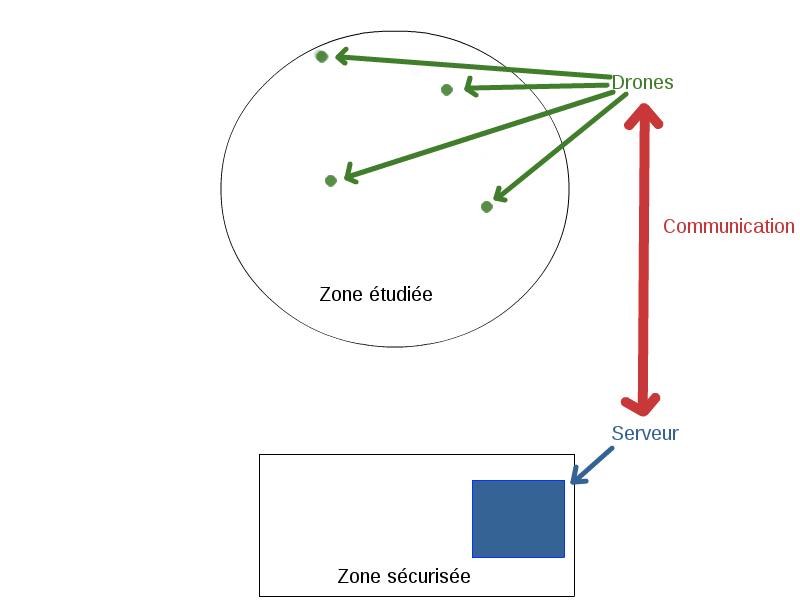
\includegraphics[scale=0.4]{img/projet_schema.png}
	  \caption{Schéma du réseau}
	  \label{network_schema}
	\end{figure}
	
	\newpage
	
	Nous avons choisi ce modèle car il répond à nos besoins et qu'il est 
plus simple à mettre en place qu'un réseau maillé par exemple. Chaque 
drone peut communiquer avec le serveur mais pas les autres drones. Et le 
serveur connait l'ensemble des drones utilisés dans l'application et peut 
donc communiquer avec eux. Aussi, si l'un des drones venait à tomber en panne 
durant une analyse, cela n'empêcherait pas le bon déroulement de l'application 
puisque le serveur pourrait continuer de communiquer avec le reste des drones, 
contrairement à une topologie en anneau par exemple (qui au passage augmenterait 
la latence de réception des données).
      
      \subsection{Fonctionnement interne du serveur}
	En ce qui concerne le fonctionnement interne du serveur nous avons 
pensé qu'il serait plus judicieux de le découper en plusieurs entités, où 
chacune d'elles serait associée à une tâche particulière. Ainsi, nous avons 
effectué le découpage suivant :

\begin{itemize}
  \item Communication
  \item Sauvegarde/Chargement des données
  \item Topographie/Décision d'ordre
\end{itemize}
	Le serveur est donc constitué de trois tâches qui tournent en 
concurrence à "l'infinie". Enfait, si nous avions fait une seule et unique 
tâche nous risquerions de perdre des données. En effet, le temps que le serveur 
traite les informations qu'il a reçu, les drones continuent de lui envoyer des 
données. Mais si le serveur n'écoute pas à ce moment là, alors ces données 
seraient perdues.
	

	\begin{figure}[htbp]
	  \centering
	  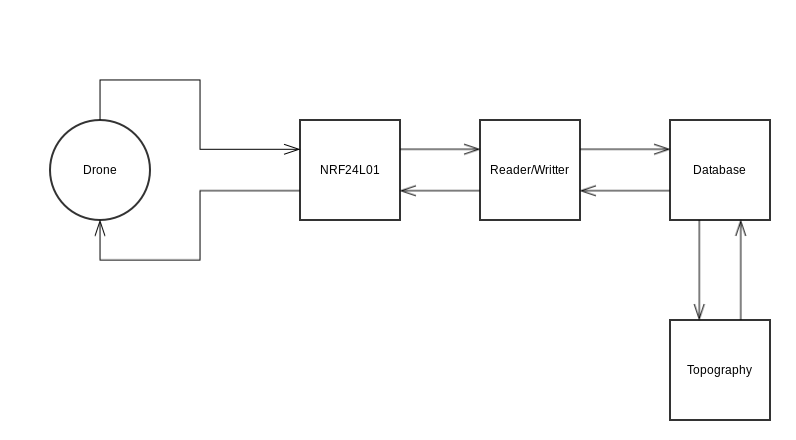
\includegraphics[scale=0.45]{img/server_model.png}
	  \caption{Transitions des données}
	  \label{server_model}
	\end{figure}
	
	La première tâche, \textit{Communication} (nommée \textit{NRF24L01} sur 
la Figure \ref{server_model}, en référence au composant utilisé pour la 
communication), se charge de lire les messages envoyés par les différents 
drones et de les réécrire sur le port série du serveur. En effet, une partie du 
serveur est constitué d'un montage à base d'\textit{Arduino} et c'est notre 
seul moyen de faire passer les données du microcontrôleur (voir section 2.1.1) 
vers le serveur. Cette même tâche se charge dans un deuxième temps de lire le 
port série, afin de vérifier s'il y a des ordres à envoyer aux drones. Si c'est 
le cas elle se charge de les communiquer aux drones concernés.

	La deuxième tâche, \textit{Sauvegarde/Chargement des données} (nommée 
\textit{Reader/Writer} sur la Figure \ref{server_model}), lit le port série du 
serveur et enregistre chaque message dans une base de données. Dans un deuxième 
temps elle accède au contenu de la base de données, afin de vérifier si des 
ordres doivent être envoyés. Si c'est le cas elle les écrit sur le port série 
afin de les transmettre à la première tâche.

	La troisième et dernière tâche, \textit{Topographie/Décision d'ordre} 
(nommée \textit{Topography} sur la Figure \ref{server_model}), récupère les 
entrées de la base de données (qui se comporte comme une pile) et les insère 
dans une matrice. Cette matrice représente la zone étudiée en vue de dessus, 
avec chacune de ses composantes représentant l'altitude aux cordonnées 
correspondantes aux indices de la composante. Ainsi, si $M_{1, 1} = 150$ (avec 
$M$ la matrice représentant la zone) cela signifie qu'au point $(1, 1)$ de la 
zone un drone a mesuré une altitude de 150 centimètres. À chaque fois 
qu'une donnée est inséré dans la matrice, cette tâche se charge de dessiner 
le nouveau contenu à l'écran. Ce qui permet à l'utilisateur de suivre en 
direct l'évolution de l'analyse, et ce de manière graphique. Dans un deuxième 
temps cette tâche analyse si un ordre doit être envoyé. Cela dépend de 
plusieurs paramètres. Par exemple, si une zone de la carte n'a pas encore été 
dévoilée le serveur peut demander à un drone de s'y rendre pour y récolter des 
informations. Ou si un drone n'a plus beaucoup de batterie, le serveur peut lui 
demander de revenir dans la zone sécurisée afin que l'utilisateur le recharge. 
Si cette troisième tâche détermine qu'un ordre doit être envoyé, alors elle 
l'écrit dans la base de données afin de le faire remonter à la seconde tâche.

	Maintenant que nous en savons un peu plus sur le principe de 
fonctionnement, nous pouvons présenter la manière dont nous avons implémenté 
cela.
    
    \section{Implémentation}
      La première tâche est constituée d'une partie matérielle et logicielle. 
La partie matérielle est un simple montage formé par une carte Arduino et un 
transmetteur/récepteur radio (voir Figure \ref{montage_serveur}).

	\begin{figure}[htbp]
	  \centering
	  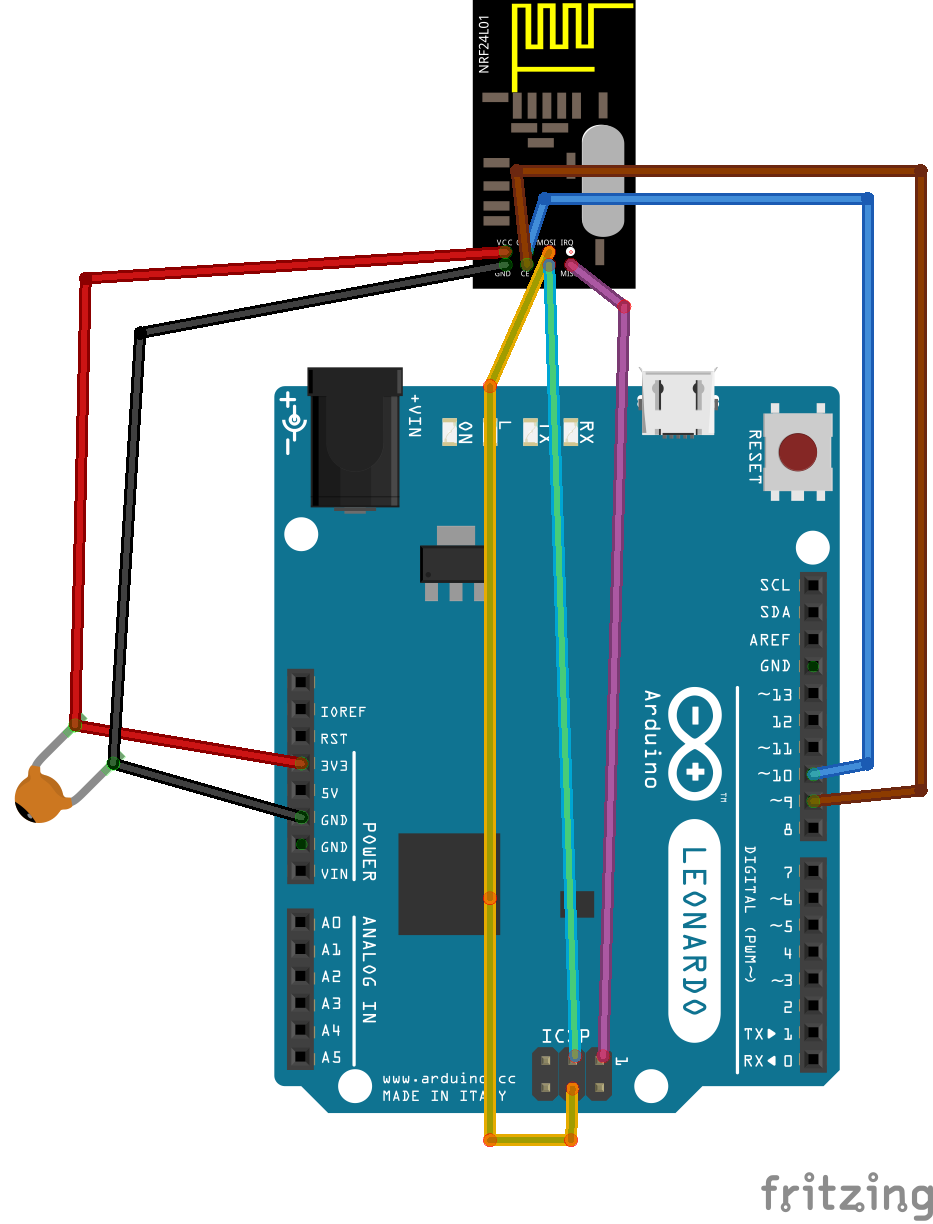
\includegraphics[scale=0.8]{img/montage_serveur.png}
	  \caption{Montage matériel du serveur}
	  \label{montage_serveur}
	\end{figure}
	
      Puisque cette tâche utilise un montage à base d'Arduino, la partie 
logicielle de cette tâche est codée dans le langage d'Arduino. Ce programme se 
contente de parcourir l'ensemble des adresses des drones connus et de lire les 
messages reçus. Un message est représenté par un tableau de la forme indiquée 
par la Figure \ref{message_drone}.

	\begin{figure}
	  \begin{center}
	    \begin{tabular}{|c|c|c|c|c|c|c|c|c|c|c|}
	      \hline
	      $d$ & $x$ & $y$ & $z$ & $s1$ & $s2$ & $s3$ & $s4$ & $s5$ & $s6$ & 
$e$ \\
	      \hline
	    \end{tabular}
	  \end{center}
	  \caption{Représentation d'un message de drone}
	  \label{message_drone}
	\end{figure}
	
	Avec :
	\begin{itemize}
	  \item $d$ : identifiant du drone
	  \item $x$ : position en abscisse
	  \item $y$ : position en ordonnée
	  \item $z$ : altitude du drone
	  \item $s1$ à $s6$ : valeurs des capteurs
	  \item $e$ : code d'état
	\end{itemize}

	La tâche se charge alors de recopier le contenu des tableaux, sur le 
port série afin de les communiquer à la deuxième tâche. Une fois l'ensemble des 
messages recopiés, elle lit le port série afin de voir si des ordres doivent 
être envoyés. Si c'est le cas, elle forme un tableau (représenté par la 
Figure \ref{message_serveur}) et le transmet au drone concerné.

	\begin{figure}
	  \begin{center}
	    \begin{tabular}{|c|c|c|c|c|}
	      \hline
	      $d$ & $x$ & $y$ & $z$ & $e$ \\
	      \hline
	    \end{tabular}
	  \end{center}
	  \caption{Représentation d'un ordre}
	  \label{message_serveur}
	\end{figure}
	
	Avec :
	\begin{itemize}
	  \item $d$ : identifiant du drone destinataire
	  \item $x$ : position cible en abscisse
	  \item $y$ : position cible en ordonnée
	  \item $z$ : altitude cible du drone
	  \item $e$ : code supplémentaire
	\end{itemize}
	
	Que ce soit pour les messages ou pour les ordres, on peut remarquer 
qu'une valeur $e$ est présente dans la dernière case du tableau. Cette valeur 
additionnelle permet de communiquer une information supplémentaire dans un 
message. Par exemple, on peut imaginer qu'un drone envoie $e = 5$ ce qui 
pourrait signifier "Je n'ai plus de batterie". Dans ce cas le serveur sait 
interpréter le cas où $e = 5$ et construirait un ordre en conséquence.

	La deuxième tâche, quant à elle, est implémentée en 
\textit{Python}\cite{python}. Nous avons choisi ce langage car nous n'avons pas 
besoin d'un langage puissant comme le \textit{C/C++} et il est moins gourmand 
que \textit{Java}. De plus, il possède une communauté énorme. Ainsi, il existe 
des bibliothèques pour tout et n'importe quoi. Le langage étant très simple de 
base, avec toutes ces bibliothèques il devient sûrement le langage le plus 
simple pour déployer de petites applications. Par exemple, il existe une 
bibliothèque pour accéder au port série de la machine, avec des fonctions très 
simples d'utilisation.

	Quand la deuxième tâche récupère un message elle doit l'insérer dans 
une base de données. Notre application ne nécessite pas la puissance du 
\textit{SQL}. En effet, tout ce que nous voulons faire ces récupérer tout le 
contenu, entrée par entrée. Ainsi, nous n'avons pas besoin de faire des 
requêtes avec des entrées classée dans un certain ordre, ou alors des requêtes 
avec des conditions, etc. C'est pour cette raison que nous avons choisi 
d'utiliser une base de données \textit{Redis}\cite{redis}. C'est une base de 
données basée sur des ensembles "clé-valeur". Ainsi, dans notre application la 
zone étudiée (la clé) sera associée à une pile de message (la valeur). Un autre 
point fort de notre choix d'implémentation est qu'il existe une bibliothèque 
pour la manipulation de Redis avec Python. 

      La troisième tâche est elle aussi implémentée en Python. Dans la section 
1.1.2 nous avons expliqué que nous représentons la zone étudiée par une 
matrice. Nous partons du principe que nous ne connaissons pas la taille de la 
zone. Ainsi, notre matrice doit être constamment redimensionnée. Il existe 
encore une bibliothèque très utile en Python, nommée 
\textit{Numpy}\cite{numpy}. C'est une bibliothèque scientifique qui propose 
divers fonctions implémentant des algorithmes connus pour le calculs 
scientifique, mais dans notre cas ce qui nous intéresse c'est les structures de 
données qu'elle propose. En effet, les matrices Numpy sont très puissantes car 
elles disposent de divers méthodes pour leur manipulation et notamment des 
méthodes de redimensionnement dynamique.
      Aussi, cette tâche doit représenter graphiquement le contenu de la 
matrice. Numpy est très souvent couplé à une seconde bibliothèque nommée 
\textit{MatPlotLib}\cite{matplotlib}. Celle-ci permet de dessiner des 
graphiques à l'écran. Elle fonctionne très bien avec Numpy puisque ses méthodes 
s'attendent déjà à recevoir des objets venant de cette dernière.

      Maintenant que nous avons présenté le fonctionnement du serveur nous 
allons pouvoir vous présenté un exemple de résultat.

    \section{Résultat}
      La Figure\ref{exemple_topo} est une capture d'écran d'une topographie que 
nous avons obtenue par le biais du serveur.

	\begin{figure}[htbp]
	  \centering
	  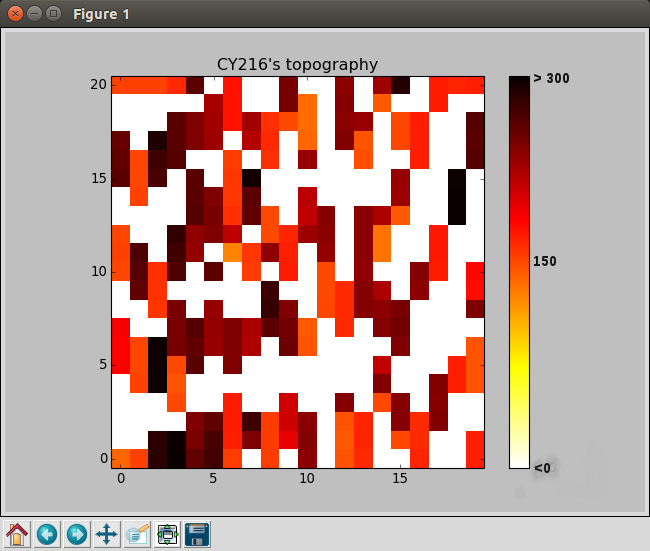
\includegraphics[scale=0.4]{img/topography_example.png}
	  \caption{Exemple de topographie}
	  \label{exemple_topo}
	\end{figure}
	
      On peut y voir un certain nombre d'éléments. Le plus visible est le 
graphique lui-même. Il représente la zone étudiée en vue de dessus. Ainsi à 
chaque coordonnée de la zone est associée une certaine hauteur. Le degré de 
cette hauteur est représenté par une couleur plus ou moins foncé. Plus cette 
couleur est foncée plus le point est élevé. Sur la droite du graphique se 
trouve sa légende. Elle indique la valeur en centimètres du degré de hauteur. 
On remarque donc que pour des points blancs cela représente le sol, et que pour 
des points noirs cela représente une hauteur de trois mètres. Cela est dû au 
fait que les capteurs ultrasons que nous utilisons pour les mesures ont une 
distance de mesure maximum. Mais le serveur lui peut fonctionner avec n'importe 
quelle valeur.

      Il faut noter que nous ne possédions pas de drone fonctionnel pour faire 
les essais du serveur. Ainsi l'exemple de topographie montré par la 
Figure \ref{exemple_topo} ne représente rien de spécial. Nous avons fournit des 
coordonnées aléatoires pour chaque point et nous avons fait varier les mesures 
du capteur en plaçant notre main devant et en jouant avec la distance.

      Dans tous les cas, lors de cet essais la réception et la représentation 
des messages se sont avérées fonctionnelles. Ainsi, si le serveur était utilisé 
avec un drone qui fournit sa véritable position et les valeurs renvoyées par 
ses capteurs, le serveur fournirait toujours les résultats attendus.

    \section{Envoi d'ordres}
      Toutefois, le serveur n'est pas encore totalement fonctionnel. Il reste 
l'envoi d'ordre à implémenter. La troisième tâche peut déterminer si une partie 
de la carte contient une zone encore non découverte. Ainsi, elle parcourt 
l'ensemble des drones et vérifie s'il existe un drone pour lequel un ordre n'a 
pas été donné (c'est-à-dire s'il existe un drone qui n'est pas en cours de 
déplacement vers une position cible). Si c'est le cas elle insère un ordre dans 
une deuxième pile Redis. La deuxième tâche lit le contenu de cette seconde 
pile. Si elle n'est pas vide elle réécrit l'ordre sur le port série du serveur. 
Cependant, nous n'arrivons pas encore à lire et écrire simultanément sur le 
port série, du côté Arduino. Donc nous ne sommes pas encore capable d'envoyer 
les ordres aux drones.

      De plus notre serveur ne détermine le besoin d'envoyer un ordre seulement 
dans le cas d'une partie encore non dévoilée de la carte. Mais il devrait être 
capable de déterminer des ordres en fonction des différents états du drone. Par 
exemple dans le cas où le drone n'a plus de batterie, pour lui demander de 
revenir à la "base". Pour établir une liste exhaustive de tous les états 
nécessitant un ordre, il nous faudrait faire des essais à l'aide d'un drone 
fonctionnel, ce que nous n'avons pas réussi à obtenir. Mais nous aborderons ce 
problème dans la suite de ce rapport.
	

  \chapter{Drone}
    Étant donné notre cursus, nous ne savions pas réellement comment procéder 
pour monter un drone. Nous avons commencé par nous renseigner sur ce qui se 
fait en matière de drones. Il faut savoir qu'il en existe de plusieurs types, 
des petits, des grands, des appareils avec un vol "agressif" (rapide et agile), 
d'autres avec un vol optimisé pour la prise de vues, certains avec un vol dit 
"hybride", etc.
    
    Pour l'application que nous voulons faire nous avons plutôt besoin d'un 
drone avec un vol hybride. Le but est de dessiner la topographie d'une zone, 
pour cela nous utilisons un capteur ultrason qui mesure la distance entre le 
drone et ce qu'il y a en dessous. Nous n'avons donc pas besoin d'un vol assez 
lent pour faire des prises de vues, mais il ne faut pas que le drone soit trop 
rapide afin de prendre le plus d'informations possible. De plus, pour des 
questions pratiques, il faut que le drone ait assez d'autonomie pour ne pas 
demander que sa batterie soit rechargée pendant une session d'analyse.
    
    Parmi les drones déjà existants, le drone \textit{Crazyflie} de chez 
\textit{Bitcraze}\cite{bitcraze} nous a intéressés par sa petite taille (voir 
Figure \ref{crazyflie}), par le fait qu'il soit libre et qu'on puisse facilement 
acheter tous les composants séparément. Nous avons donc décidé de baser notre 
modèle sur ce petit drone. Plus concrètement, le nôtre a une taille similaire 
au Crazyflie et dispose de la même batterie, des mêmes moteurs et des mêmes 
pales mais le reste des composants sont différents. Nous ne voulions pas passer 
directement par un Crazyflie, car un de nos objectifs est de construire le robot 
de A à Z. De plus ce modèle n'est pas tout à fait adapté à ce que nous voulons 
faire, car il est trop léger et est alors trop véloce. Aussi il ne possède 
pas de capteur pour récolter des informations sur la zone survolée. Donc dans 
tous les cas nous aurions été obligés de le modifier.
    
    \begin{figure}[htbp]%Photo du crazyflie
      \centering
      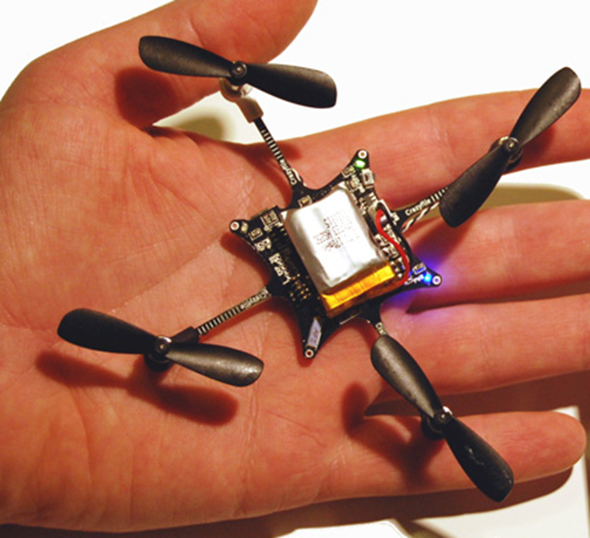
\includegraphics[scale = 0.25]{img/crazyflie.png}
      \caption{Crazyflie}
      \label{crazyflie}
    \end{figure}
    
    \section{Composants}
      L'objectif de cette section est de présenter les différents composants 
que nous avons utilisés pour construire ce premier drone.
      
      \subsection{Microcontrôleur}
	Un microcontrôleur est un \textit{system on chip}, c'est-à-dire que 
c'est une petite carte électronique proposant un certain nombre de 
fonctionnalités et pouvant fonctionner seule. C'est souvent un micro-processeur 
monté sur une carte avec plusieurs broches sur lesquelles l'utilisateur peut y 
connecter d'autres composants. Ainsi il peut réaliser un montage complexe qu'il 
pourra utiliser en programmant le micro-processeur.
	Au début de notre année scolaire, nous avons eu un séminaire de cours 
pour nous apprendre le langage \textit{Arduino}. Nous avons pu découvrir un 
langage vraiment simple à prendre en main lorsque l'on a déjà quelques bases en 
programmation avec des langages comme le \textit{C}, ou le \textit{C++}. Nous 
nous sommes donc tournés vers les technologies proposées par \textit{Arduino} 
pour le choix du microcontrôleur. Finalement, nous avons opté pour une 
\textit{Arduino Pro Mini}. Le principal intérêt de cette carte se trouve dans 
sa petite taille et sa légèreté, 18 sur 33 millimètres pour seulement deux 
grammes. De plus elle propose un nombre suffisant de broches pour l'ensemble de 
notre montage.
	
	\begin{figure}
	  \begin{subfigure}{.5\textwidth}
	    \centering
	    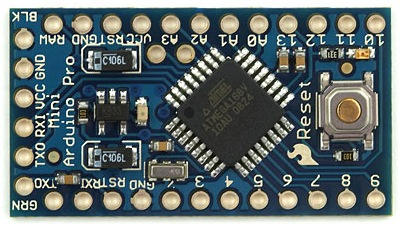
\includegraphics[scale=0.2]{img/arduinopromini.jpg}
	    \caption{Image de l'Arduino Pro Mini}
	    \label{imagearduino}
	  \end{subfigure}%
	  \begin{subfigure}{.5\textwidth}
	    \centering
	    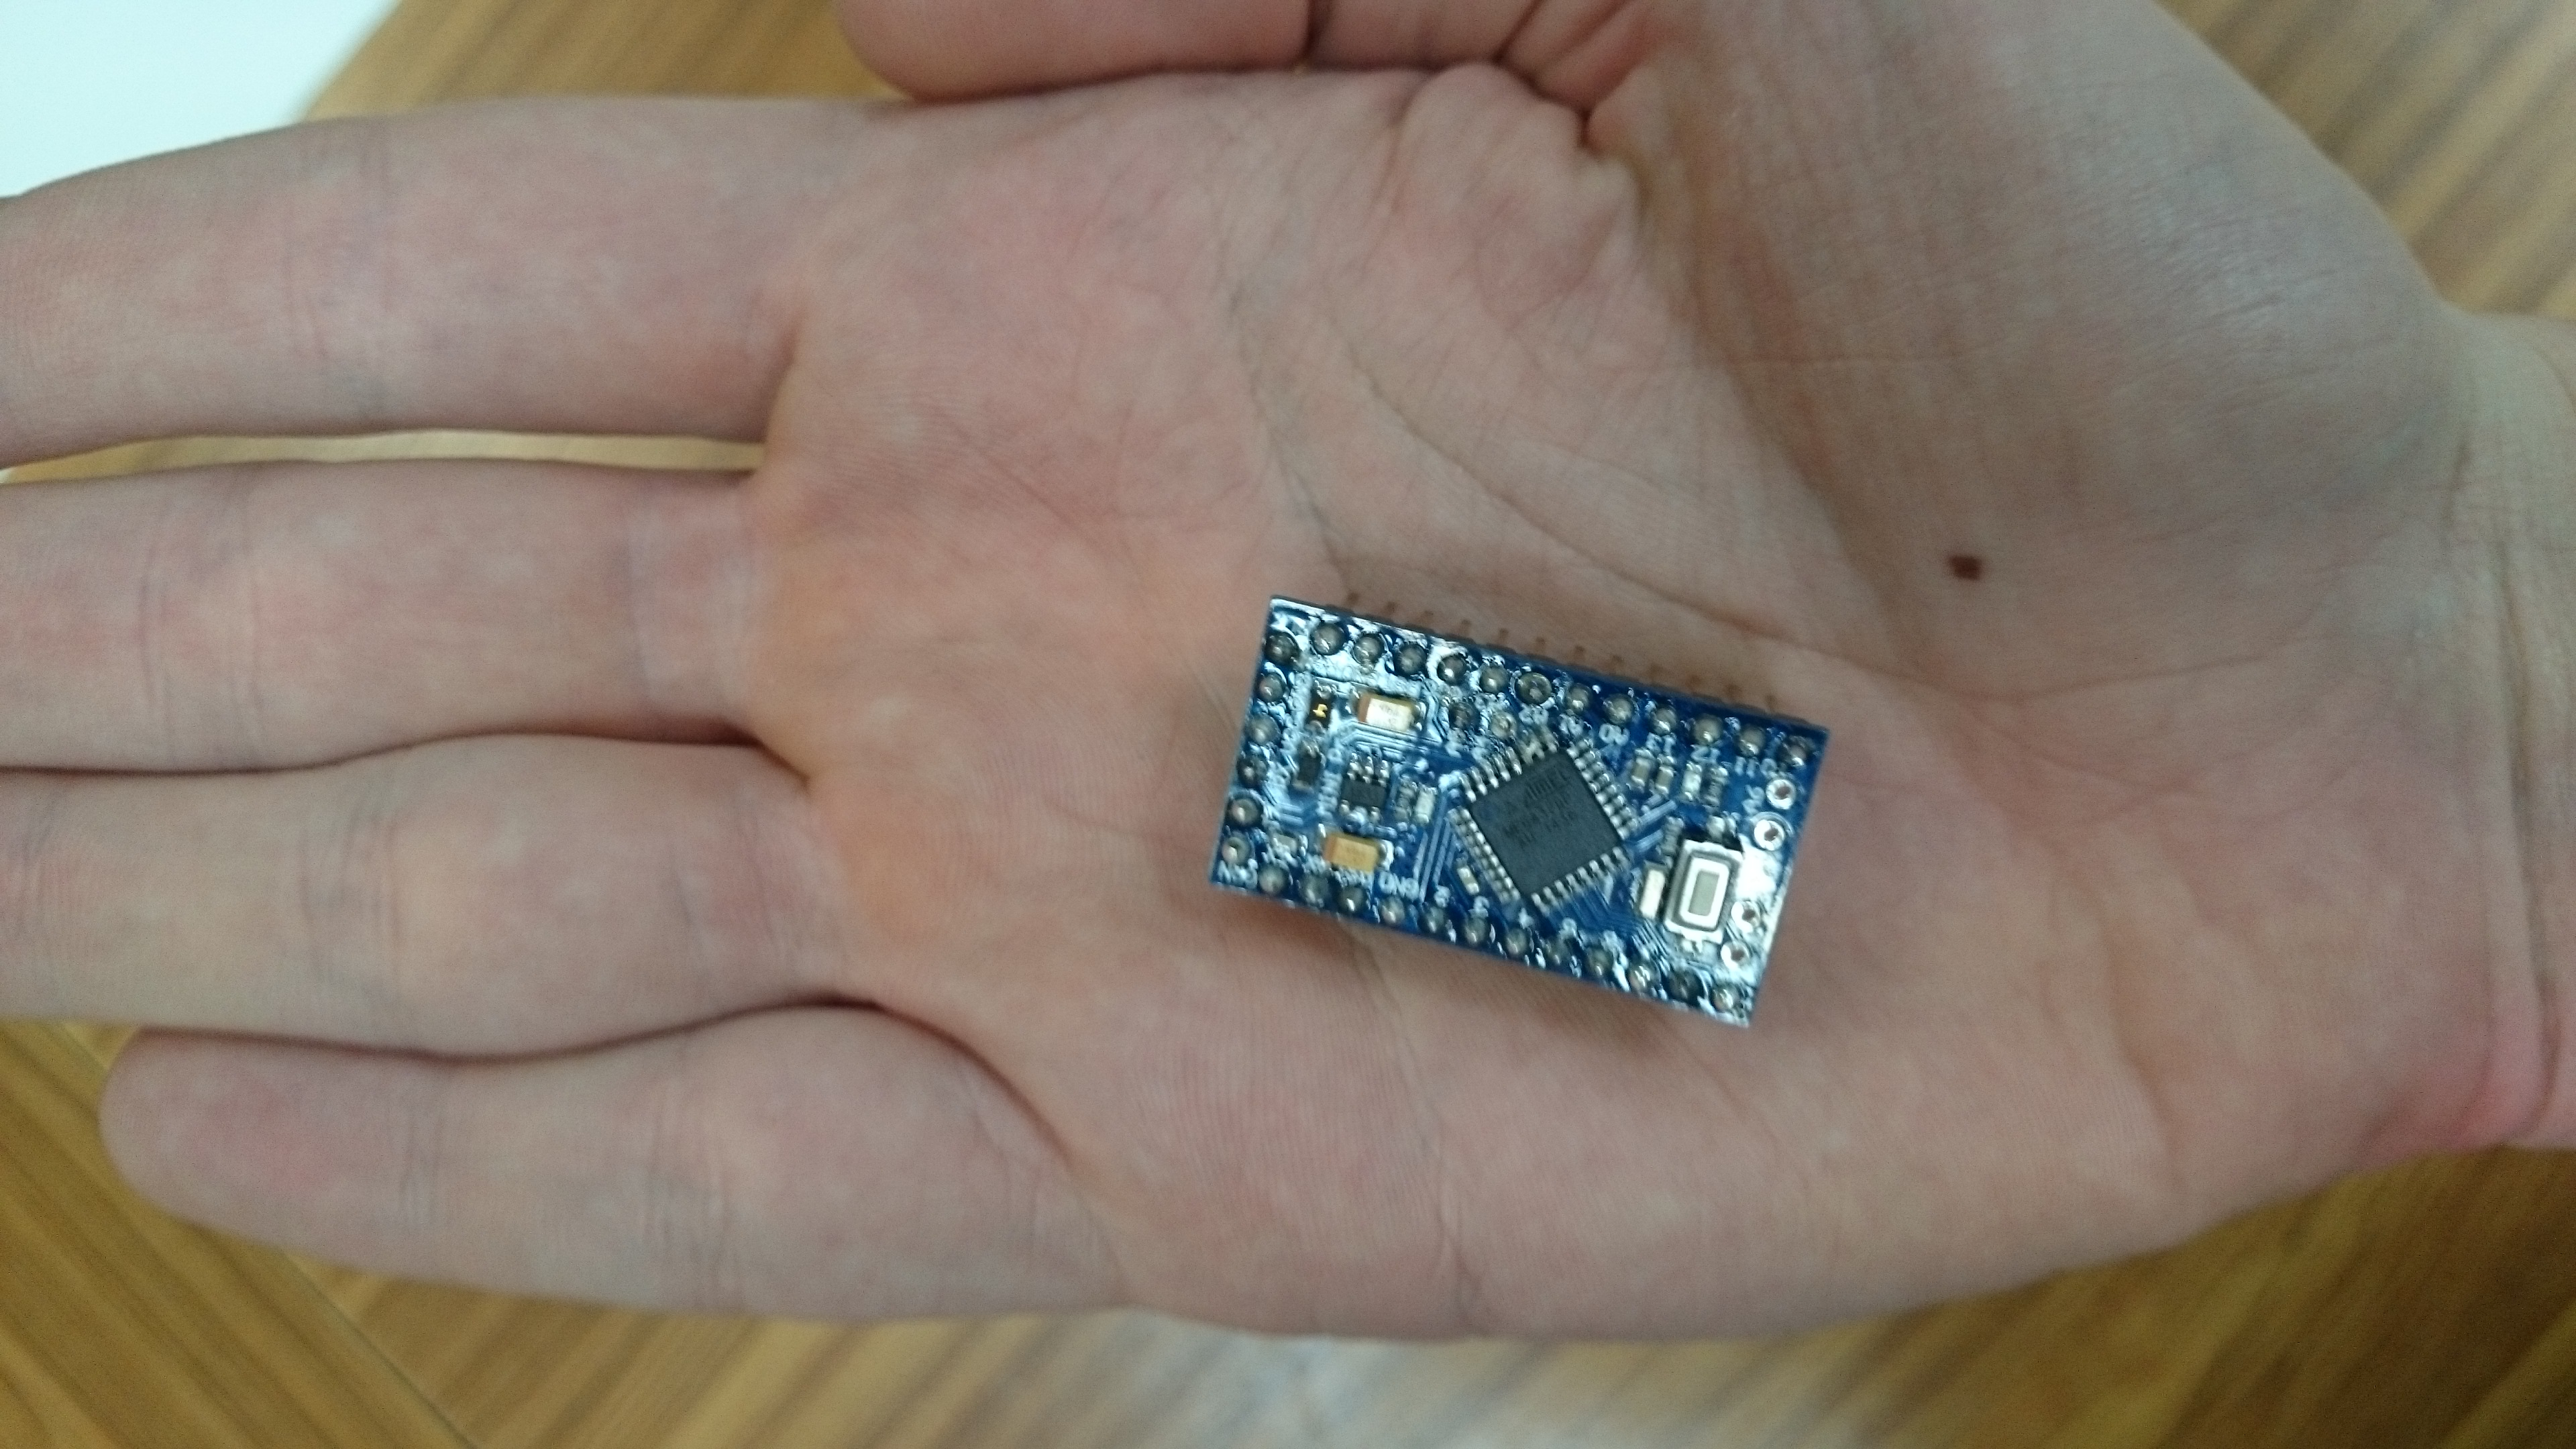
\includegraphics[scale=0.06]{img/arduino.JPG}
	    \caption{Photographie de notre Arduino Pro Mini}
	    \label{photoarduino}
	  \end{subfigure}
	  \caption{Image et photographie de l'Arduino Pro Mini}
	  \label{arduino}
	\end{figure}
	
      Une fois le microcontrôleur en main, il nous faut ajouter d'autres 
composants nécessaire à la mise en place d'un drone. En branchant ces 
composants dans les trous sur l'extérieur de la carte nous pourrons les 
contrôler de manière logicielle, en codant le microprocesseur grâce au langage 
Arduino. Le microprocesseur, lui, se chargera de les faire fonctionner 
physiquement.  
	
      \subsection{Equilibrage et localisation}
	Il est important de disposer d'une technologie pour assister le drone à 
se stabiliser. Pour cela, ce dernier doit connaître "en permanence" son angle 
d'inclinaison. Nous avons donc besoin d'un gyroscope. Le large catalogue de 
modules \textit{Arduino} propose une pièce qui fournit un gyroscope et un 
accéléromètre, le \textit{MPU-6050} (voir Figure \ref{mpu6050}). Ce module a 
une taille et un poids similaires à ceux du microcontrôleur, 25.5 sur 15.2 
millimètres pour 1.5 grammes. Un autre point fort de ce circuit est qu'il est 
très utilisé au sein de la communauté Arduino. Il est donc facile de trouver 
des exemples d'utilisation.
	
	Pendant un certain moment nous nous sommes demandé comment nous 
pourrions connaître la position de notre drone dans l'espace. Naturellement 
nous avons pensé au GPS, mais la précision de ces technologies (pour rester dans 
un budget abordable) n'est clairement pas assez précise. Bien entendu, dans le 
cadre où le drone devrait faire son analyse en extérieur sur une zone assez 
grande, les GPS sont intéressants. Mais notre drone devra simplement analyser 
une salle de classe, alors une précision "au mètre près" est beaucoup trop 
large. Nous aurions plutôt besoin d'une précision de l’ordre du décimètre.  Une 
autre solution a été évoquée, créer notre propre système de localisation, en 
créant une triangulation\cite{triangulation} à l’aide d’un réseau d’antennes. 
Ce principe consiste à placer trois antennes autour d'une zone et qui emmettent 
un signal. L'objet qu'on souhaite localiser réceptionne ces signaux et calcul 
sa position dans l'espace en fonction de sa position par rapport à l'ensemble 
des émetteurs. Toutefois, pour des raisons de coûts cette solution ne nous 
semble pas viable sur notre drone. Aussi, elle n'est pas conforme à la 
problématique de notre projet, puisque nous partons du principe que nous ne 
connaissons pas l'étendue de la zone. Ainsi, nous ne pourrions pas placer nos 
antennes.

	Finalement une connaissance, nous a conseillé de travailler avec un 
accéléromètre. Un accéléromètre est un module permettant de mesurer 
l'accélération linéaire d’un système. En connaissant l'accélération de notre 
drone, il sera alors possible de déterminer sa vitesse et donc, ses déplacements 
dans l’espace. Nous avons donc choisi de nous tourner vers cette solution. 
C'est aussi pour cette raison que nous avons choisi le MPU6050 car il embarque 
un accéléromètre.
	
	    \begin{figure}
	      \begin{subfigure}{.5\textwidth}
		\centering
		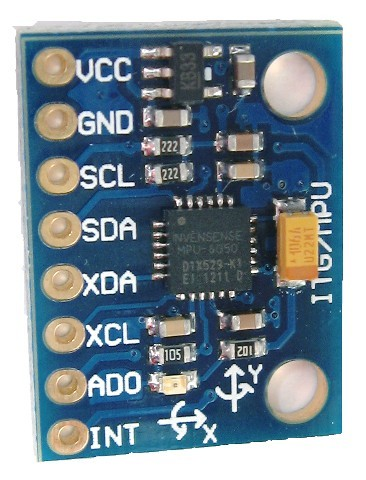
\includegraphics[scale=0.2]{img/mpu-6050.jpg}
		\caption{Image du MPU6050}
		\label{imagempu6050}
	      \end{subfigure}%
	      \begin{subfigure}{.5\textwidth}
		\centering
		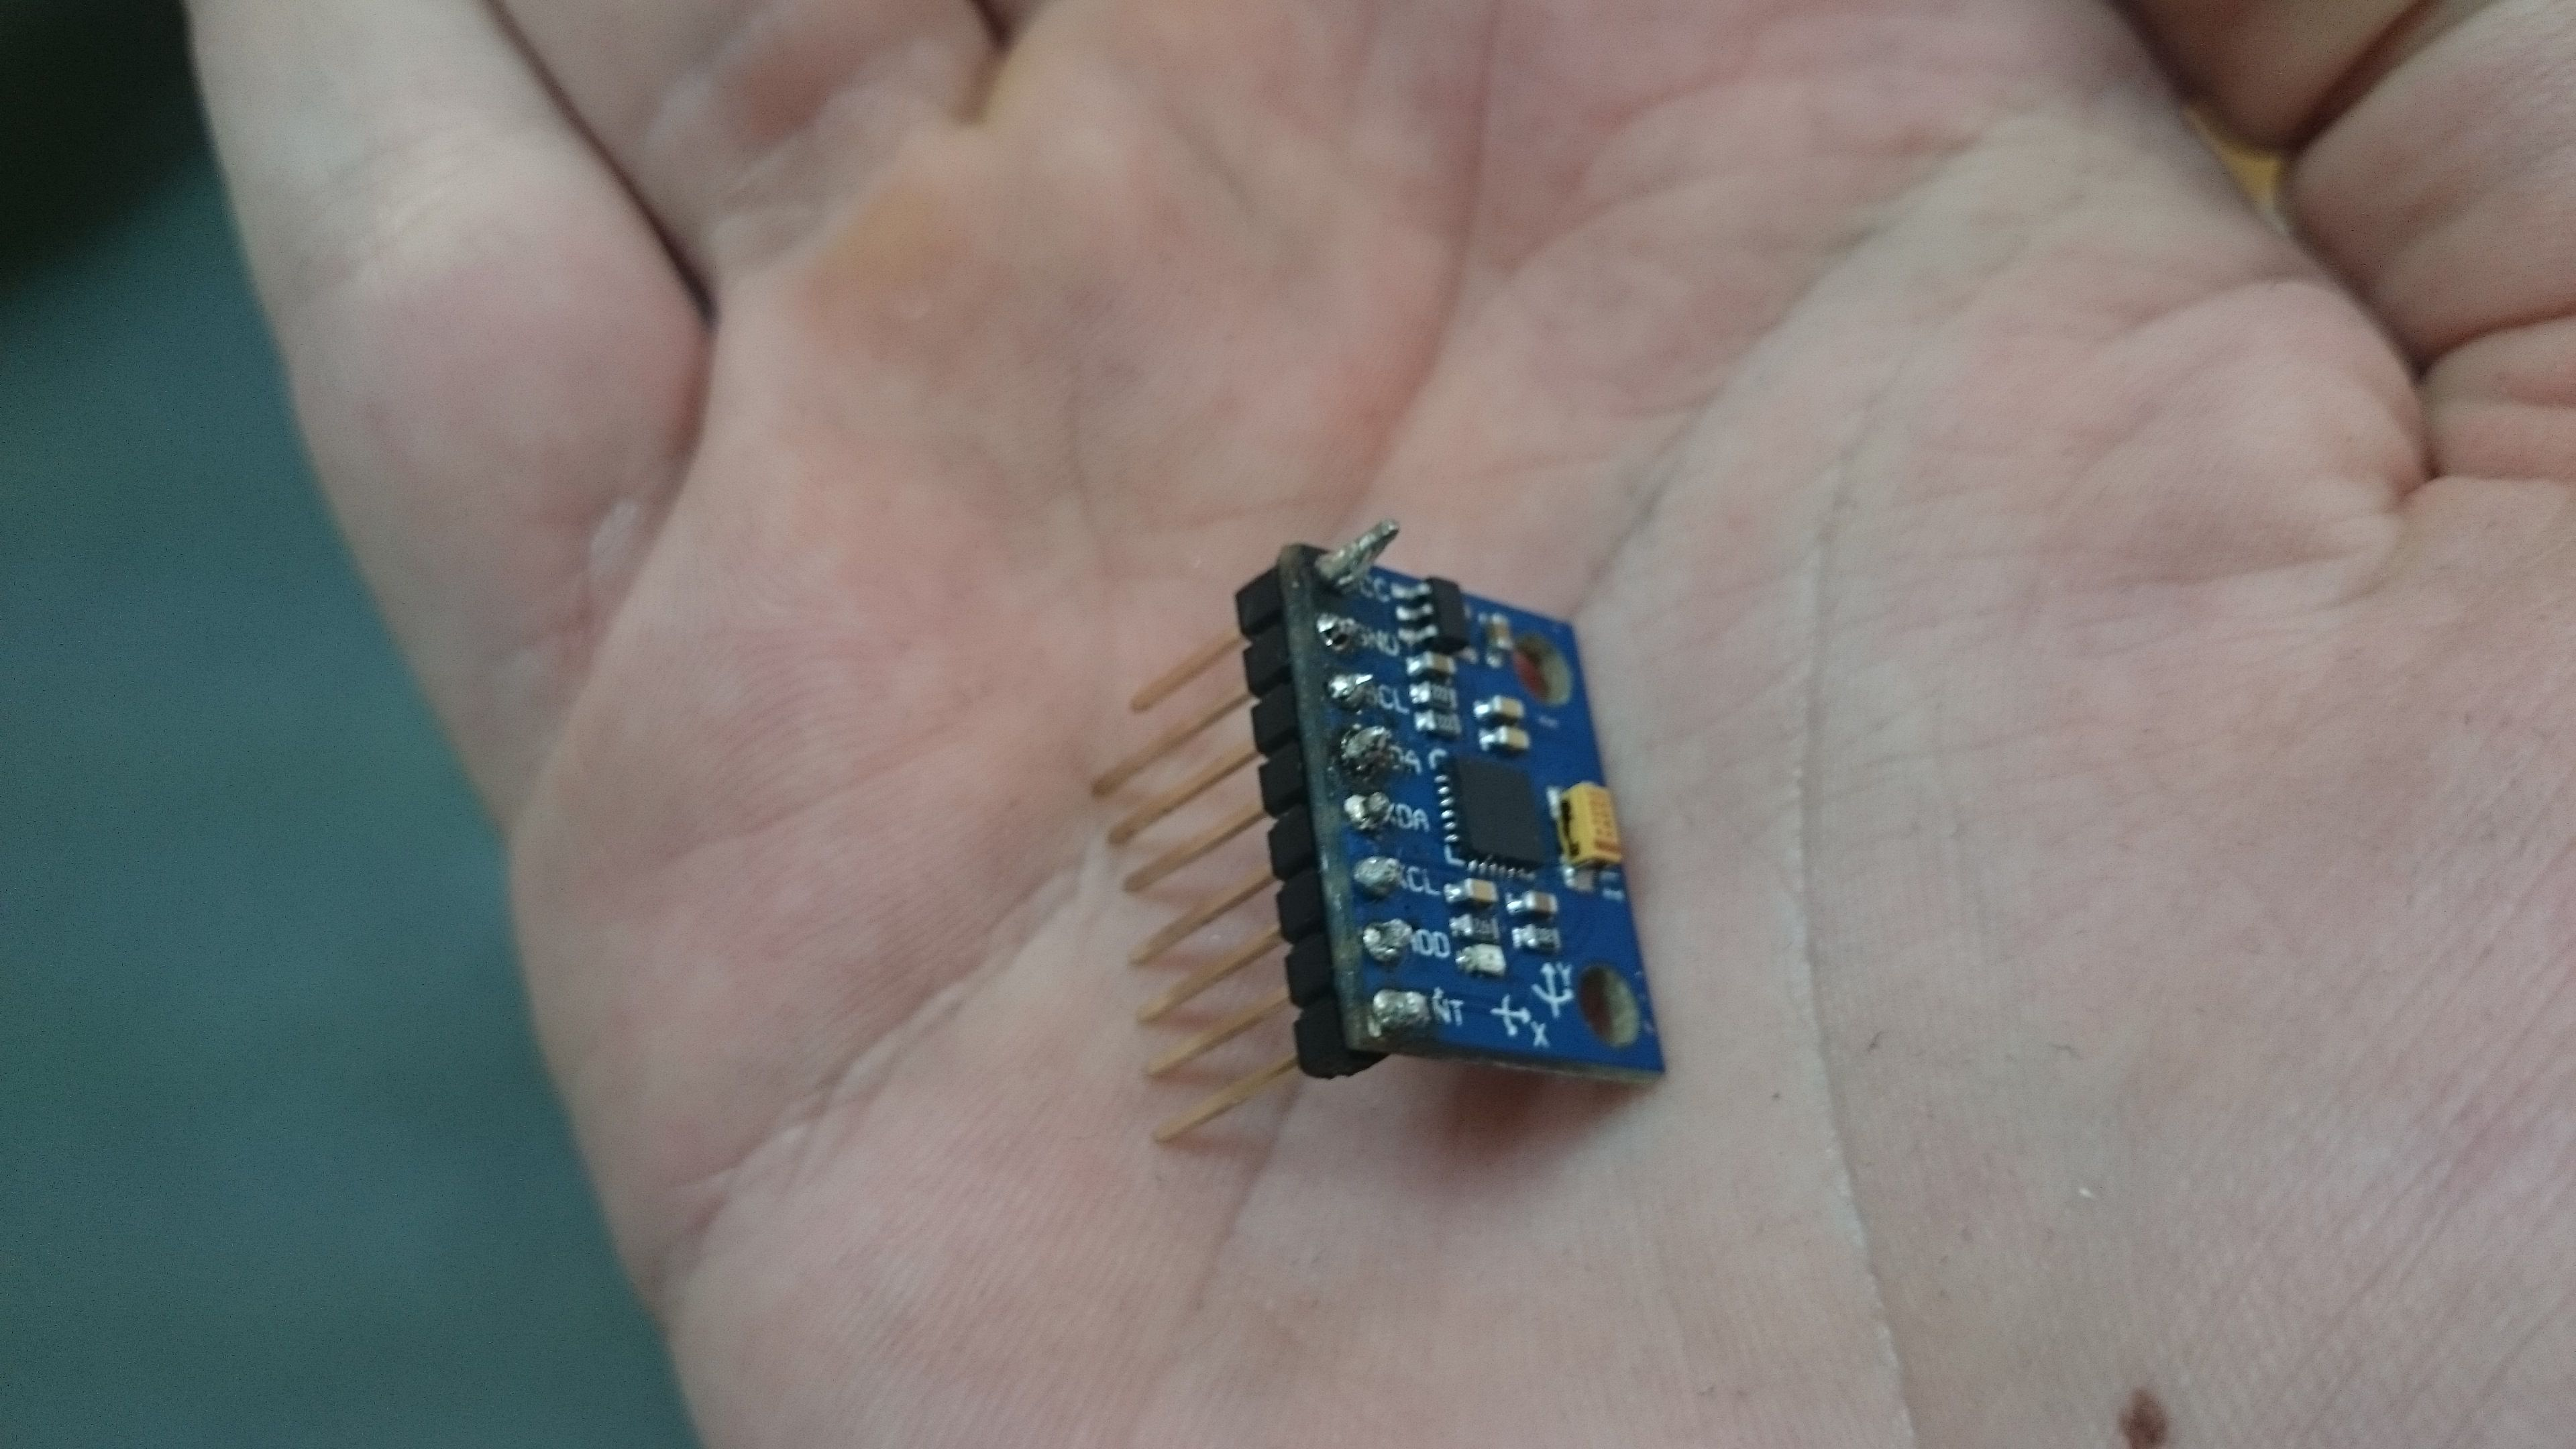
\includegraphics[scale=0.06]{img/mpu6050.jpg}
		\caption{Photographie de notre MPU6050}
		\label{photompu6050}
	      \end{subfigure}
	      \caption{Image et photographie du MPU6050}
	      \label{mpu6050}
	    \end{figure}
	    
	Pour pouvoir utiliser ce composant nous avons utilisé la bibliothèque 
développée par Jeff Rowberg\cite{jeff_rowberg_lib}. Ses travaux permettent de 
représenter logiciellement un gyroscope et de récupérer les valeurs calculées 
par le MPU6050. Ainsi, en récupérant ces mesures nous pouvons déterminer la 
puissance requise pour chaque moteur afin d'équilibrer le drone.

	En cours de développement nous nous sommes rendu compte que déterminer 
la position du drone dans l'espace avec seulement un accéléromètre n'est pas 
une solution envisageable. En effet, afin de calculer cette position il faut 
intégrer deux fois les mesures renvoyées par le capteur. Or, à chaque 
intégration s'introduit une petite erreur. Mais la double intégration fait que 
nos calculs suivent une erreur quadratique. Ainsi, il nous serait peut-être 
possible de déterminer correctement une première position, mais au fil de 
l'exécution de l'application, nos calculs seraient complètement faussés. Il 
faut savoir que la problématique de déterminer la position dans l'espace d'un 
objet en mouvement dans un endroit fermé est encore au stade de la recherche. 
Cette problématique pourrait faire un sujet de projet de fin d'études à elle 
toute seule.
      
      \subsection{Communication avec le serveur}
	Afin que le drone puisse communiquer avec le serveur nous avons dans un 
premier temps pensé à utiliser des modules \textit{XBee}, qui utilisent le 
protocole de communication sans fil, défini par le standard \textit{IEEE 
802.15.4} et qui sont très répendus au sein de la communauté Arduino. De plus 
il semblerait que ces composants soient très simples d'utilisation et que la 
qualité des signaux soit très fiable. Toutefois, les modules \textit{XBee} 
sont relativement chers (23 \euro) dû au fait que le protocole utilisé soit 
breveté, nous nous sommes alors penchés vers une autre technologie. Nous avons 
finalement opté pour un module de transmission/réception radio à fréquence 
2.4GHz (voir Figure \ref{nrf24l01}). Ils sont eux aussi très répendus chez les 
utilisateurs d'Arduino. Comme pour les autres composants que nous avons 
choisis, il est bon marché (0.8 \euro) et d'une taille de 15 sur 29 millimètres 
pour deux grammes.
	
	    \begin{figure}
	      \begin{subfigure}{.5\textwidth}
		\centering
		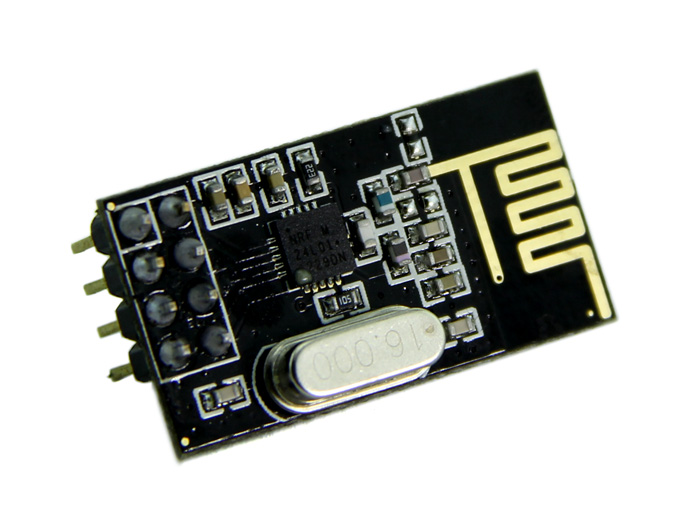
\includegraphics[scale=0.4]{img/image_nrf24l01.jpg}
		\caption{Image du NRF24L01}
		\label{imagenrf24L01}
	      \end{subfigure}%
	      \begin{subfigure}{.5\textwidth}
		\centering
		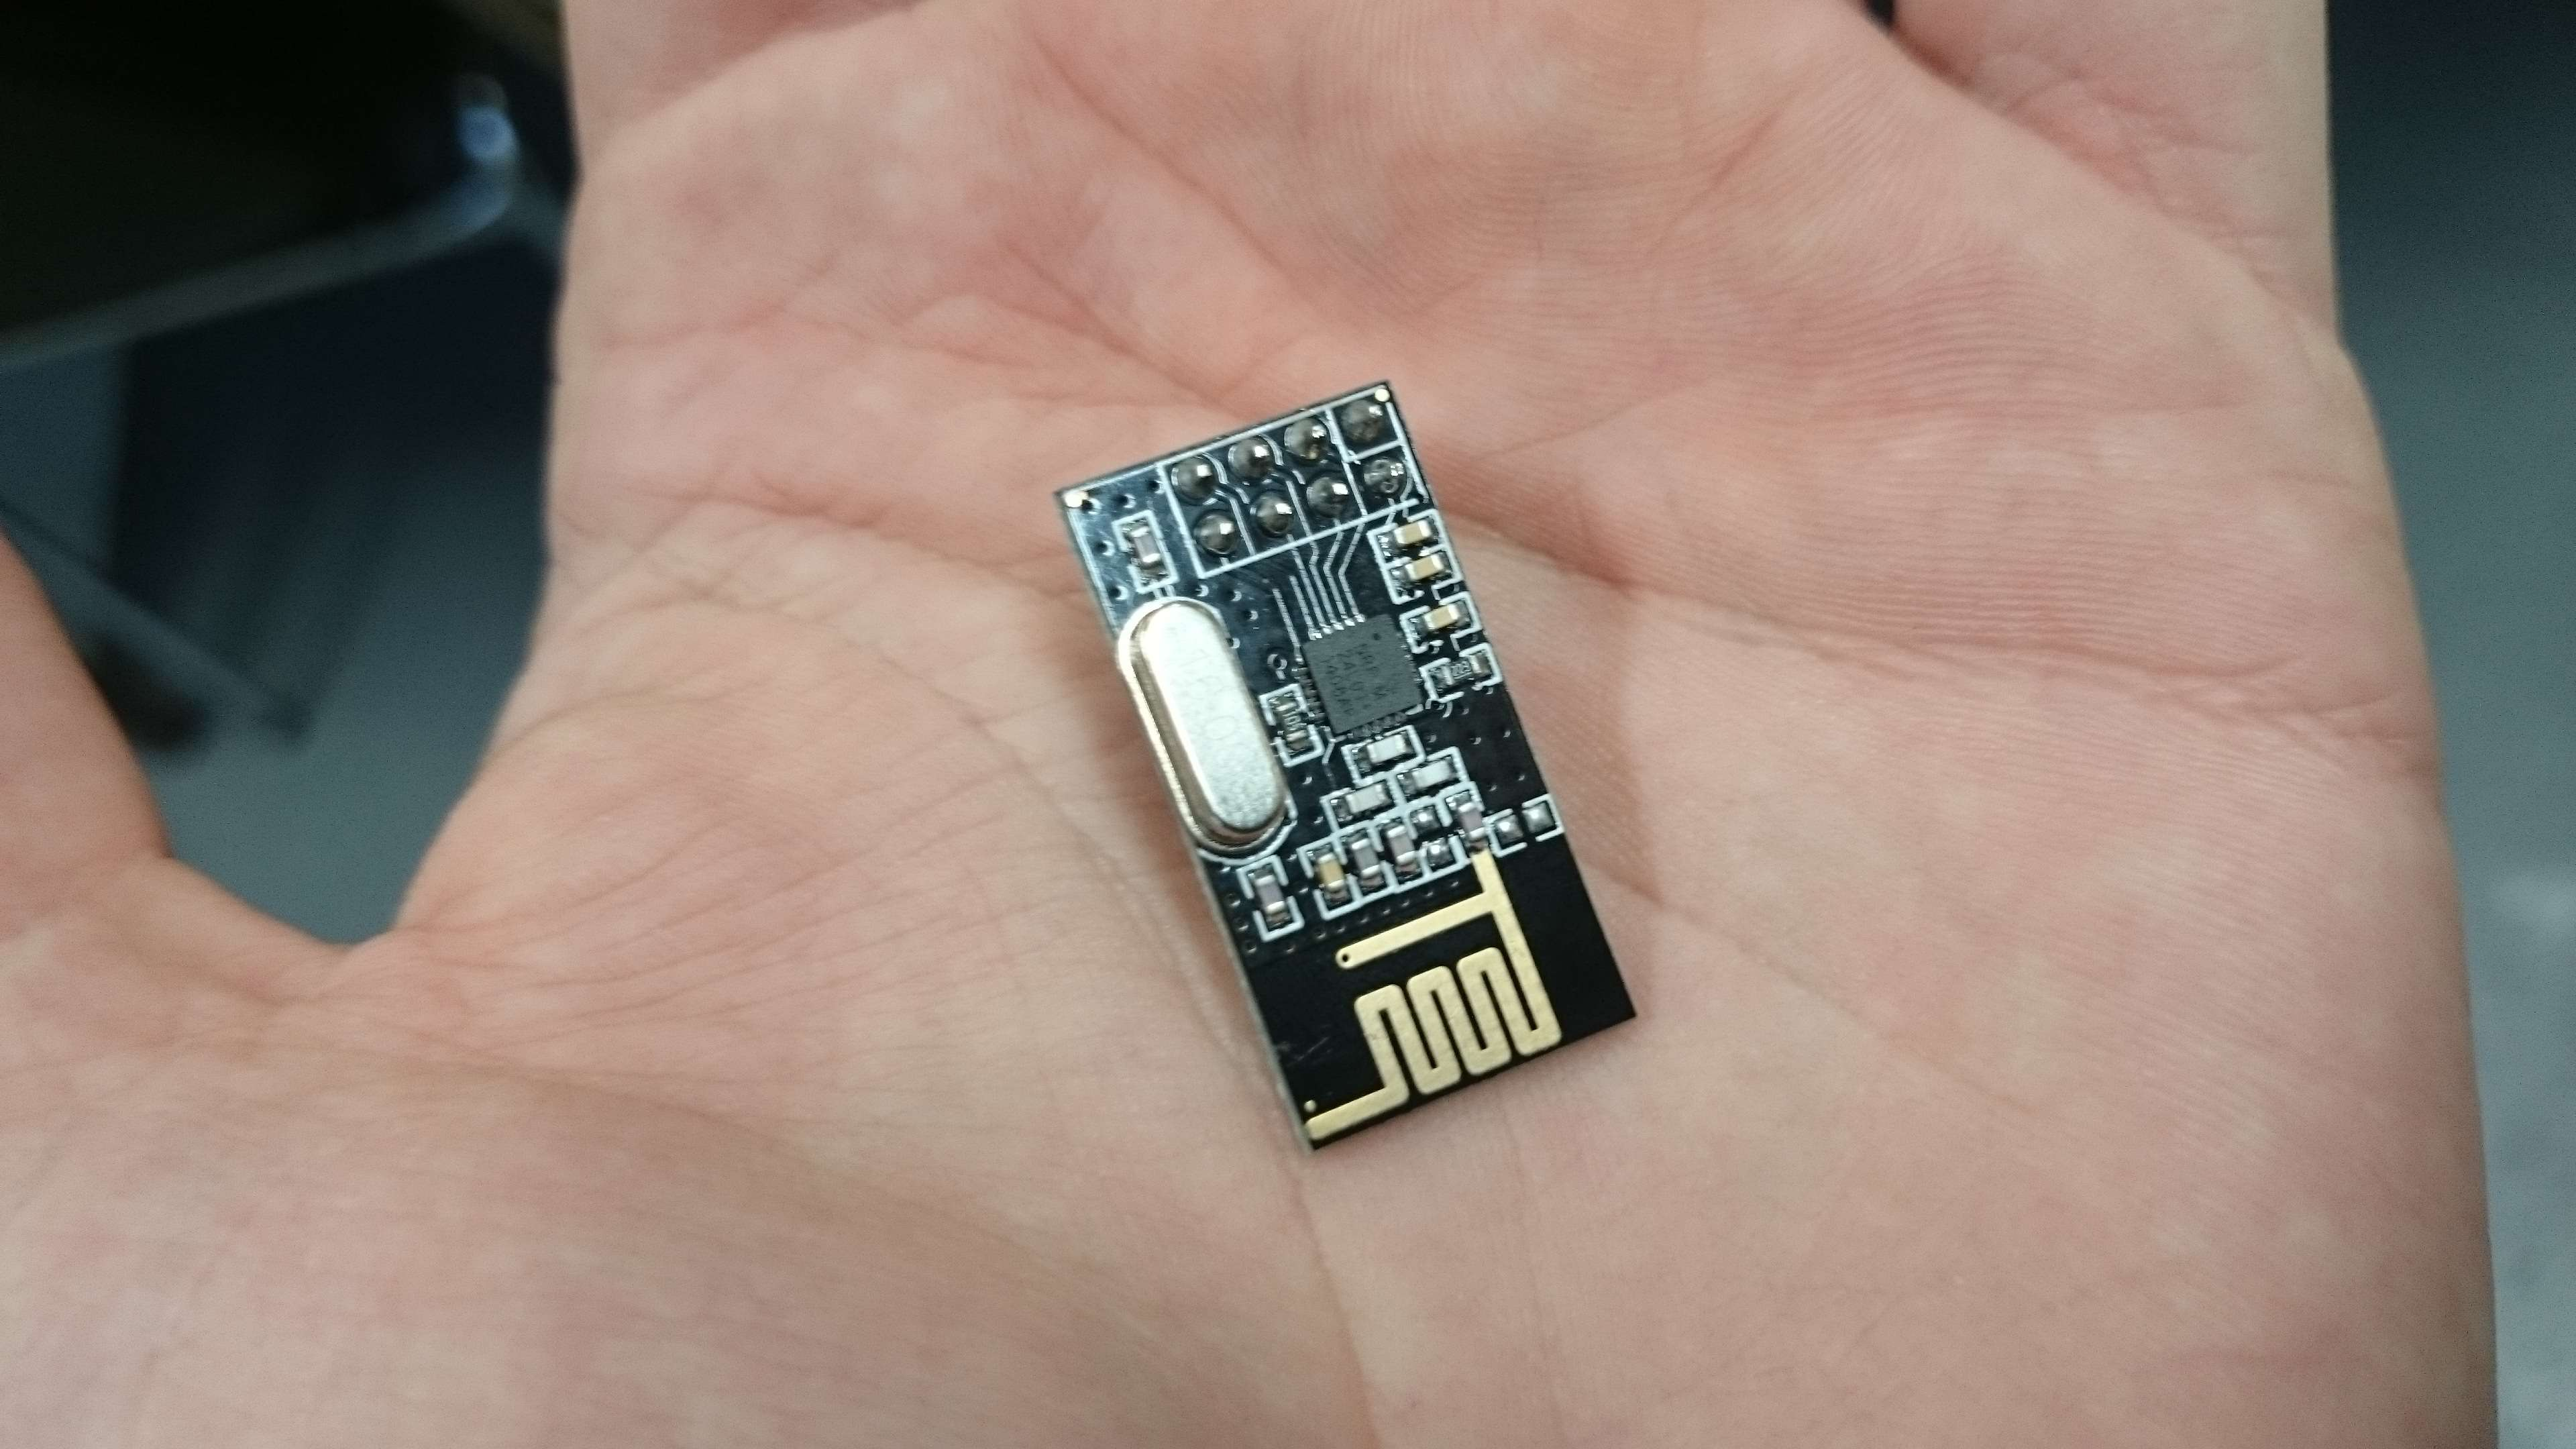
\includegraphics[scale=0.06]{img/nrf24l01.jpg}
		\caption{Photographie de notre NRF24L01}
		\label{photonrf24L01}
	      \end{subfigure}
	      \caption{Image et photographie du NRF24L01}
	      \label{nrf24l01}
	    \end{figure}
	    
	Cependant ces composants sont un peu plus compliqués à prendre en main. 
Mais heureusement, il existe de nombreuses bibliothèque. Nous avons donc créé 
une surcouche de la bibliothèque \textit{RadioHead}\cite{radiohead}. Cette 
bibliothèque permet de représenter logiciellement un transmetteur radio. À 
partir de cet objet il est possible d'envoyer et lire des messages en 
fournissant une adresse (qui représente un port entre le transmetteur et le 
récepteur qui une autre instance de ce composant, sur une autre plaquette 
Arduino). Notre surcouche nous permet de vérifier le bon envoi et la bonne 
réception des données en retournant un code d'erreur en cas d'échec.

	Toute fois le très faible coût de ces composants se ressent directement 
sur la fiabilité de leur signaux. En effet, l'envoi et la réception des données 
est malheureusement un peu aléatoire. Il n'est pas rare de ne recevoir qu'un 
message sur deux.
	
      
      \subsection{Contrôle moteur}
	La plupart des drones embarquent un \textit{Electronic Speed Controler} 
(\textit{ESC}) pour chaque moteur. Ces composants servent à contrôler la 
vitesse du moteur ainsi que son sens de rotation. Il faut savoir qu'un ESC vaut 
environ 16 \euro. Ce qui fait 64 \euro \space pour un quadcopter. Outre le prix 
important de ces modules, leur poids (25 grammes/module) aussi nous oblige à 
nous orienter vers une autre solution. Nous avons donc pensé à créer nos propres 
ESC simplement en branchant un transistor entre chaque moteur et les broches de 
sortie de l’Arduino. Les transistor on pour propriété de fonctionner comme des 
interrupteur électrique. Ainsi en couplant les variations du signal électrique 
généré par l'Arduino et la propriété du transistor nous obtenons un ESC fait 
main.

      \subsection{Moteurs}
	Dans l'introduction nous avons expliqué que nous utilisons les mêmes 
moteurs que ceux du Crazyflie. Cependant, comme pour les autres composants il 
faut coder en Arduino leur contrôle. Ainsi nous avons implémenté une petite 
bibliothèque permettant de représenter logiciellement parlant, un moteur. Cet 
objet possède alors une méthode permettant de modifier sa vitesse. Vitesse qui 
sera alors modifié logiciellement puis physiquement.

      \subsection{Mesure de la topographie}
	Pour mesurer une distance il existe plusieurs types de capteur 
différents, comme par exemple un laser. Cependant, nous ne possédons pas ce 
genre d'outil mais lors du séminaire d'Arduino du début d'année nous avons 
utilisé des capteurs ultrason (\textit{HC-SR04}). Pour ce projet nous avons 
donc choisi de réutiliser ces capteurs (pour des raisons économiques). 
Toutefois, dû aux propriétés du déplacement d'une onde sonore dans l'espace, ce 
genre de capteur n'est pas ce qu'il y a de plus fiable. L'onde sonore se 
répendant sous une forme d'arc de cercle, on ne peut pas savoir avec certitude 
quel point précisément à été mesuré.

	\begin{figure}[htbp]%Photo de l'Arduino
	  \centering
	  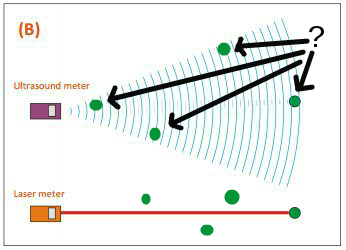
\includegraphics[scale = 0.5]{img/sonarwave.png}
	  \caption{Comparaison des fiabilités de mesure}
	  \label{sonarwave}
	\end{figure}
	
	Mais dans le cadre de la présentation de notre application ce problème 
ne sera pas vraiment dérengeant.
	
	\begin{figure}
	  \begin{subfigure}{.5\textwidth}
	    \centering
	    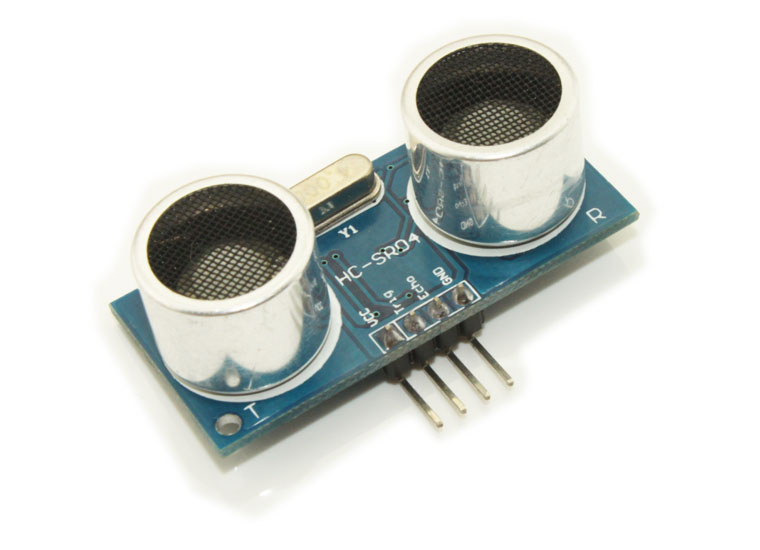
\includegraphics[scale=0.2]{img/image_hcsr04.jpg}
	    \caption{Image du HC-SR04}
	    \label{imagehcsr04}
	  \end{subfigure}%
	  \begin{subfigure}{.5\textwidth}
	    \centering
	    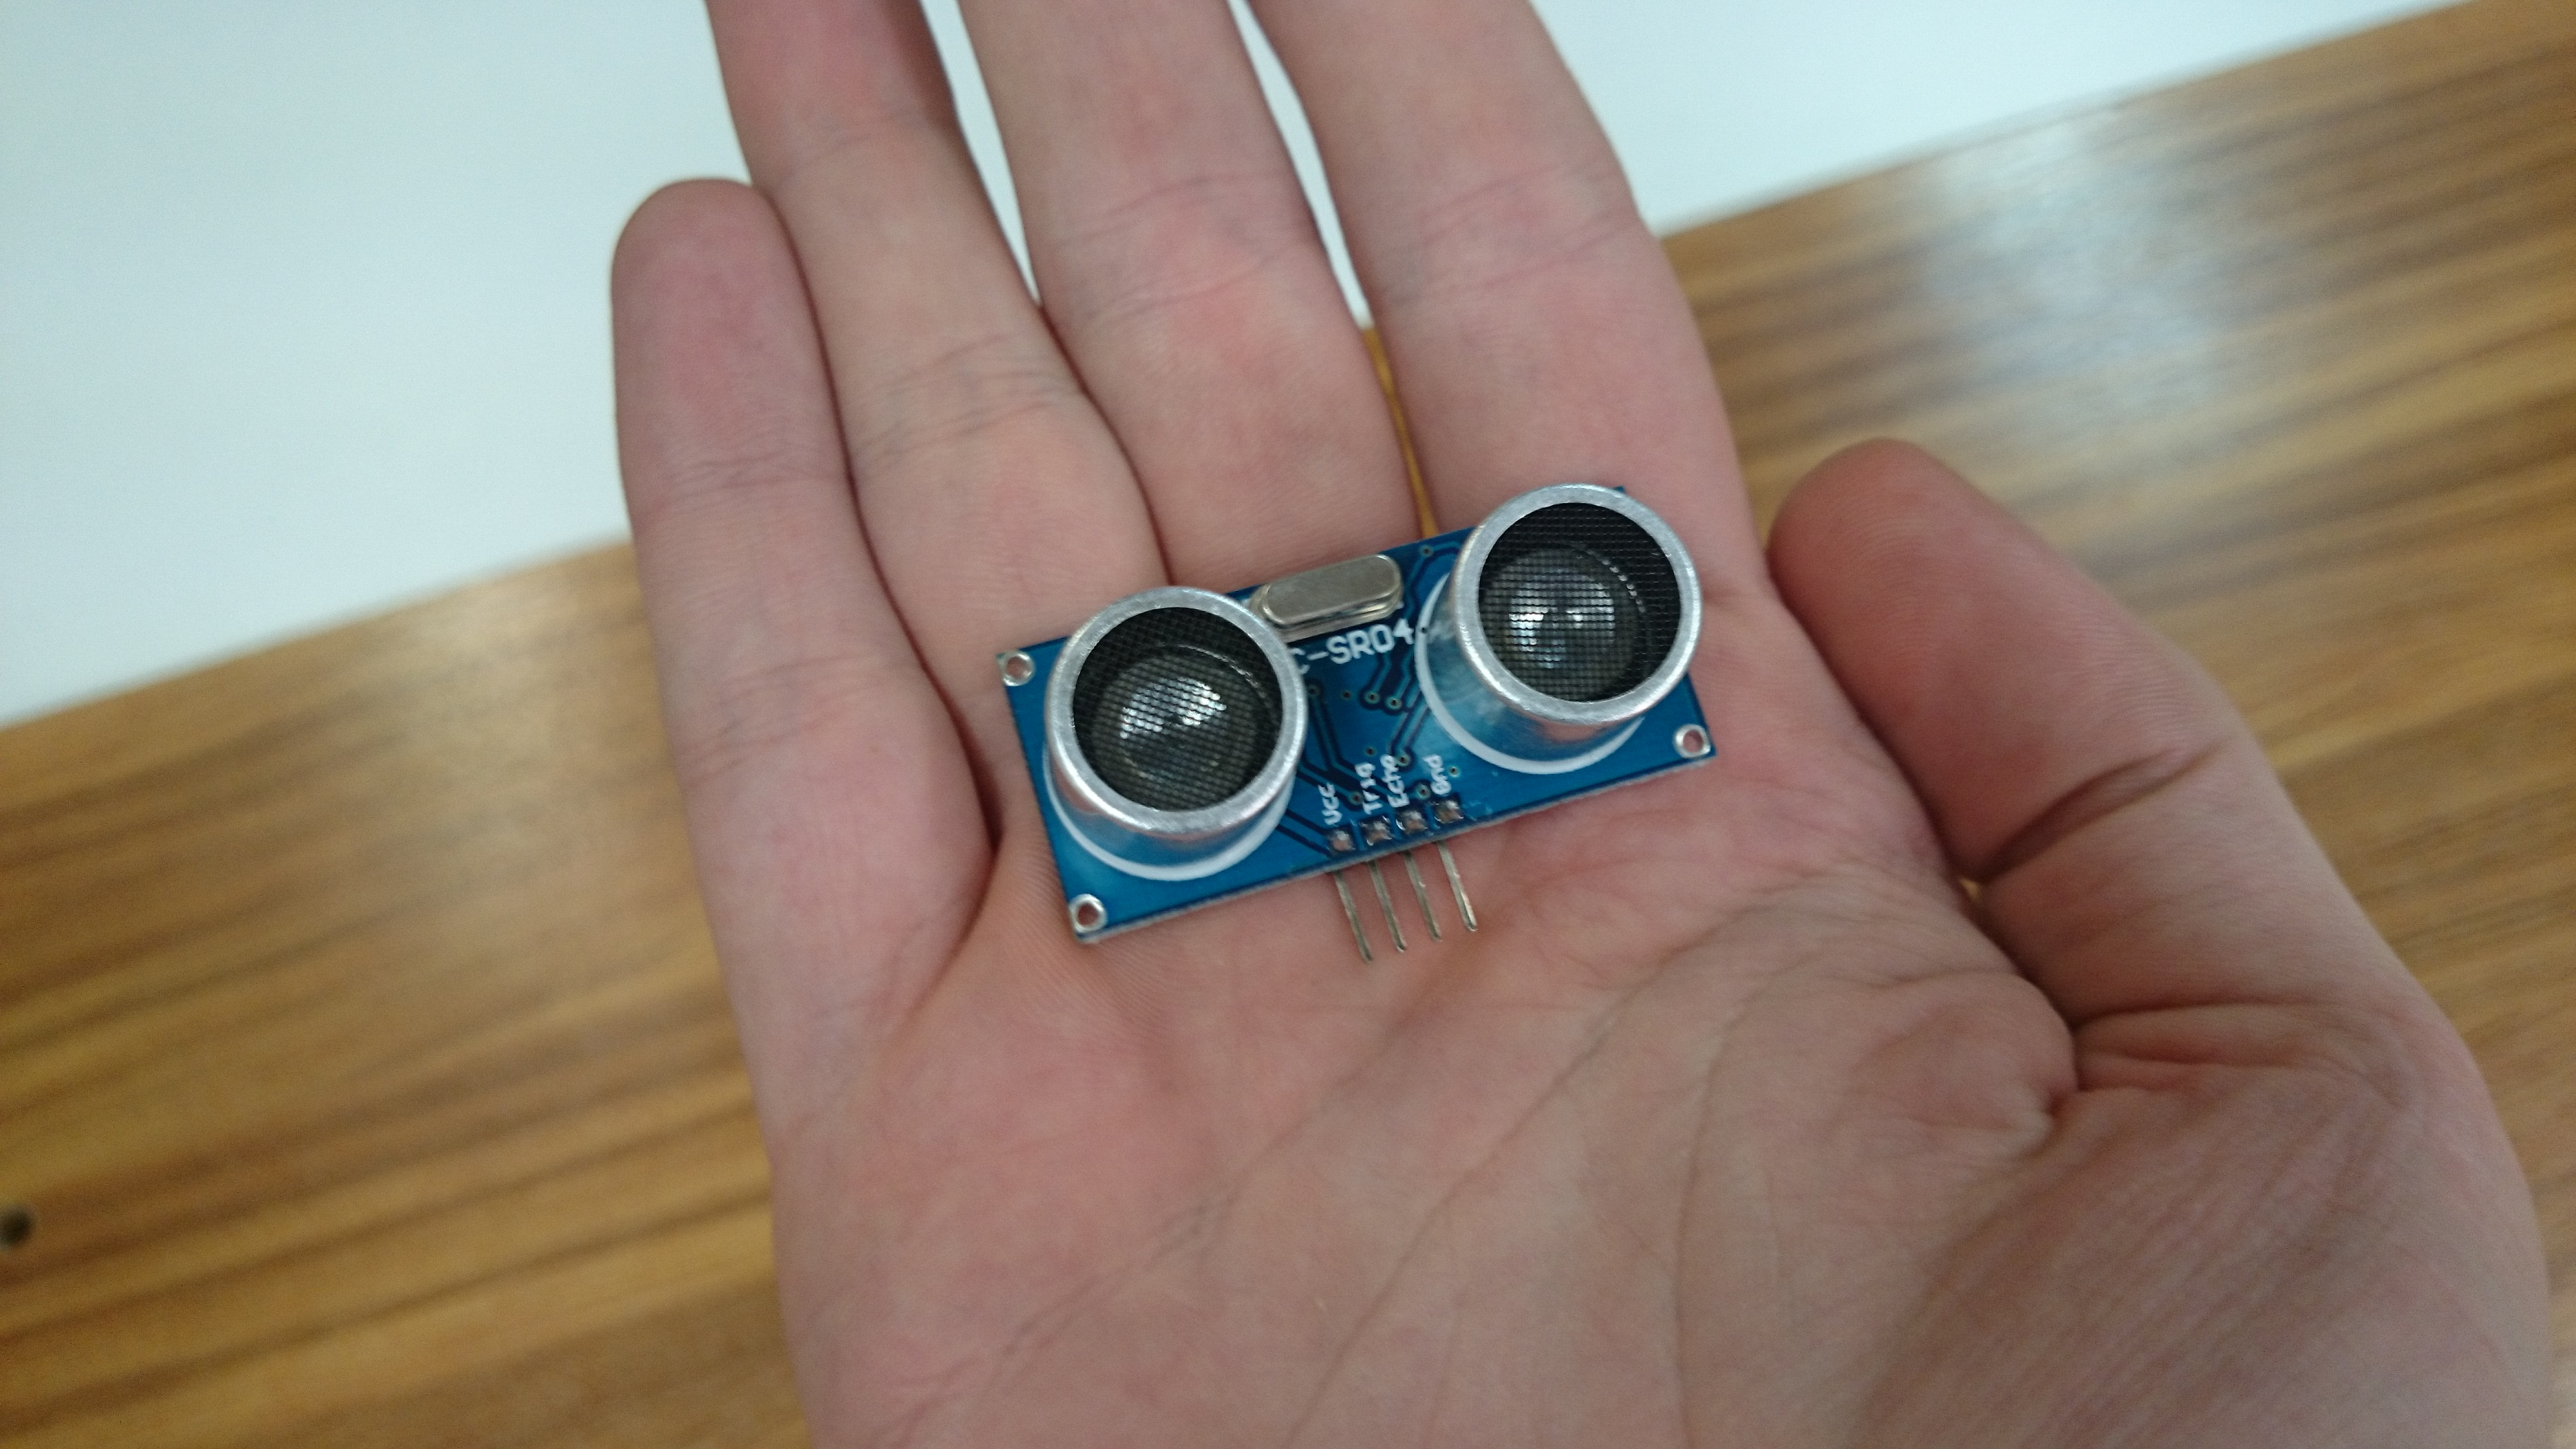
\includegraphics[scale=0.06]{img/hcsr04.JPG}
	    \caption{Photographie de notre HC-SR04}
	    \label{photohcsr04}
	  \end{subfigure}
	  \caption{Image et photographie du HC-SR04}
	  \label{hcsr04}
	\end{figure}
	
	Le HC-SR04 (voir Figure \ref{hcsr04}) est lui aussi un composant très 
répendu au sein de la communauté Arduino. Ainsi nous pouvons directement 
utiliser une bibliothèque déjà implémentée, \textit{NewPing}\cite{newping}. 
Elle permet de représentée logiciellement un capteur ultrason et de calculer la 
distance d'un point par rapport au montage en mesurant le temps de retour de 
l'onde sonore.
	
    \section{Assemblage}
      Une fois tous les composants reçus et une fois toutes les bibliothèques 
développées nous avons pu assembler le tout. Toutefois, il restait encore deux 
pièces manquantes au puzzle. En effet, il manquait encore le circuit qui relit 
tous les composants à l'Arduino et un moyen de fixer les moteurs au drone. 
Cependant ces deux éléments ne sont pas des articles que l'on peut acheter sur 
un site de vente. Nous allons expliquer dans cette section comment nous avons 
obtenu ces deux dernières pièces et présenter le résultat après assemblage.

      \subsection{Circuit}
	Pour pouvoir assembler tous les composants ensemble il faut réaliser un 
circuit imprimé. Pour cela nous avons utilisé le logiciel 
\textit{Fritzing}\cite{fritzing}. C'est un logiciel libre qui permet de 
réaliser des schémas électroniques ainsi que le PCB associé (c'est à dire le 
dessin qui va servir à la production du circuit). Ce logiciel propose de base 
un large catalogue de composants mais il est aussi possible de créer les siens. 
Aussi, un grand nombre de personnes utilisent ce logiciel, ce qui permet dans 
la plupart des cas de ne pas avoir à créer de composants puisqu'il y a de 
grandes chances que des utilisateurs les aient déjà dessinés.

      \begin{figure}[htbp]%PCB du premier drone
	\centering
	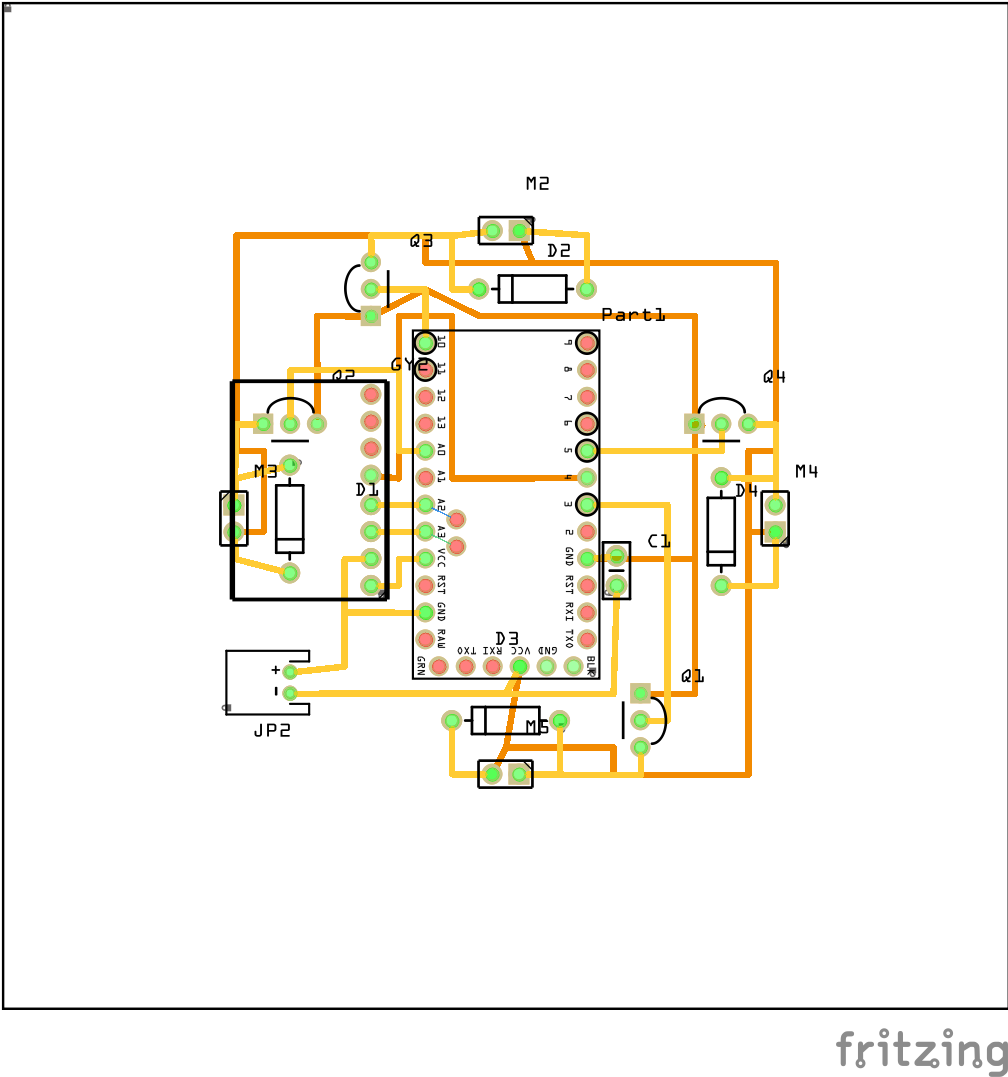
\includegraphics[scale = 0.9]{img/nouveau_drone_circuit_pcb.png}
	\caption{PCB du drone}
	\label{pcb1drone}
      \end{figure}
      
      La Figure \ref{pcb1drone} représente le PCB de notre drone. C'est le type 
de dessin qui servent à la production de circuits imprimés. Le dessin d'un PCB 
est une étape obligatoire dans la production d'un montage électronique car un 
circuit dépend du résultat attendu. Le montage entre un drone et un ordinateur 
ne sera pas le même et même le montage entre un drone et un autre modèle de 
drone sera différent. C'est pour cette raison qu'on ne peut pas acheter un 
circuit déjà fait.
      
      \subsection{Fixations moteur}
	Comme nous nous sommes inspirés du Crazyflie, nous avons fait le choix 
de ne pas utiliser de châssis. Ces composants sont assez compliqués à choisir, 
car il faut choisir entre un matériau léger mais coûteux et un matériau "lourd" 
et bon marché. Donc nous avons pensé que le circuit pourrait lui-même faire 
office de châssis. Bien entendu, ce choix est risqué car le drone est plus 
fragile. Mais notre application n'est pas vraiment "à risque" dans le sens où 
notre drone n'est pas censé faire des acrobaties et que nous comptions mettre en 
place des sécurités pour qu'il évite les obstacles de son environnement.

	De plus les moteurs du Crazyflie ont une dimension assez particulière. 
Habituellement les moteurs de drone sont plus gros ainsi il serait difficile de 
trouver un châssis qui soit compatible avec nos moteurs. De plus, souvent les 
moteurs de drone se vissent sur le châssis, mais les moteurs du Crazyflie ne 
possèdent pas de pas de vis. Nous étions donc dépendant de la solution utilisé 
par le Crazyflie, c'est à dire utiliser des petites pièces en plastique qui se 
chargent de fixer les moteurs au circuit imprimé.

	Ces fixations ne sont pas disponibles à la vente. Cependant, BitCraze a 
déposé le fichier de modélisation sur leur compte GitHub\cite{gitbit}. Ainsi, 
nous avons pu télécharger ce fichier afin de le fournir à une imprimante 3D 
pour produire les pièces qu'il nous fallait.

      \begin{figure}[htbp]%PCB du premier drone
	\centering
	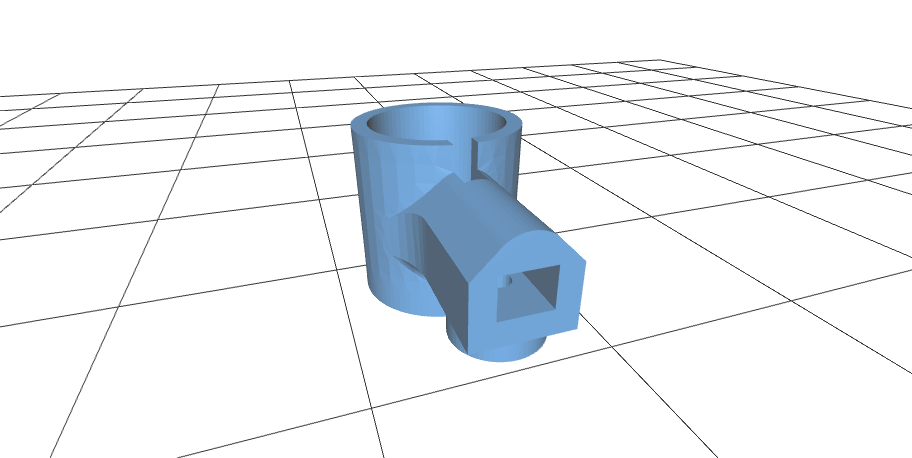
\includegraphics[scale = 0.4]{img/model_fixation.png}
	\caption{Modèle de fixation moteur}
	\label{fixationmodel}
      \end{figure}
      
	La Figure \ref{fixationmodel} est une capture d'écran du fichier de 
modélisation des fixations moteurs.

      \subsection{Production des pièces manquantes}
	L'EISTI étant une école d'ingénieur informatique, elle ne dispose ni 
du matériel nécessaire pour la production de circuit imprimé, ni d'imprimante 
3D pour imprimer nos fixations moteur. Ainsi, nous avons dû chercher une entité 
externe à notre école pour pouvoir obtenir nos deux dernières pièces. 

	Dans un premier temps nous avons pensé à nous servir du 
fablab\cite{faclab} de l'université de Cergy-Pontoise. Cet atelier se trouve à 
Gennevilliers (92), il propose un grand nombre d'outils mis à disposition 
gratuitement. La seule contrepartie est de donner de son temps à la vie du 
laboratoire. Toutefois pour utiliser certaines machines comme les imprimantes 
3D (de qualité), les découpeuses lazer, les fraiseuses, etc... il est 
nécessaire de suivre une formation. Les gérants étant conscients que nous 
sommes soumis à des deadlines, nous ont proposé de faire les choses à notre 
place. En échange nous devions simplement faire des formations sur 
l'utilisation du logiciel Fritzing et sur la fabrication d'un drone. Ils nous 
ont alors demandé de leur envoyer un mail afin qu'on puisse rester en contact. 
Ce que nous avons fait au retour de notre visite. Cependant, nous n'avons 
jamais obtenu de réponse.

      Nous avons alors cherché un autre moyen. Il existe des entreprises qui 
disposent de quelques imprimantes 3D. Elles les mettent alors à disposition du 
public contre une petite somme d'argent. Nous avons envoyé une commande, à 
l'aide du fichier de modélisation. Mais notre demande s'est vue être refusée 
car leurs imprimantes ne sont pas assez précises pour nos besoins.

      À cette même époque, notre école accueillait le concours annuel de 
robotique, \textit{RobAFIS}\cite{robafis}. Durant la compétition des 
entreprises exposaient leurs produits. Notamment \textit{Polytech 
Instrumentation}\cite{polytechinstru} (une filiale de 
\textit{Jeulin}\cite{jeulin}) exposait des imprimantes 3D. Nous en avons alors 
profité pour leur demander s'ils accepteraient de nous imprimer nos pièces. Ils 
ont alors accepté et nous avons reçu nos pièces (voir Figure \ref{fixation}) 
par courrier deux semaines plus tard.

      \begin{figure}[htbp]%PCB du premier drone
	\centering
	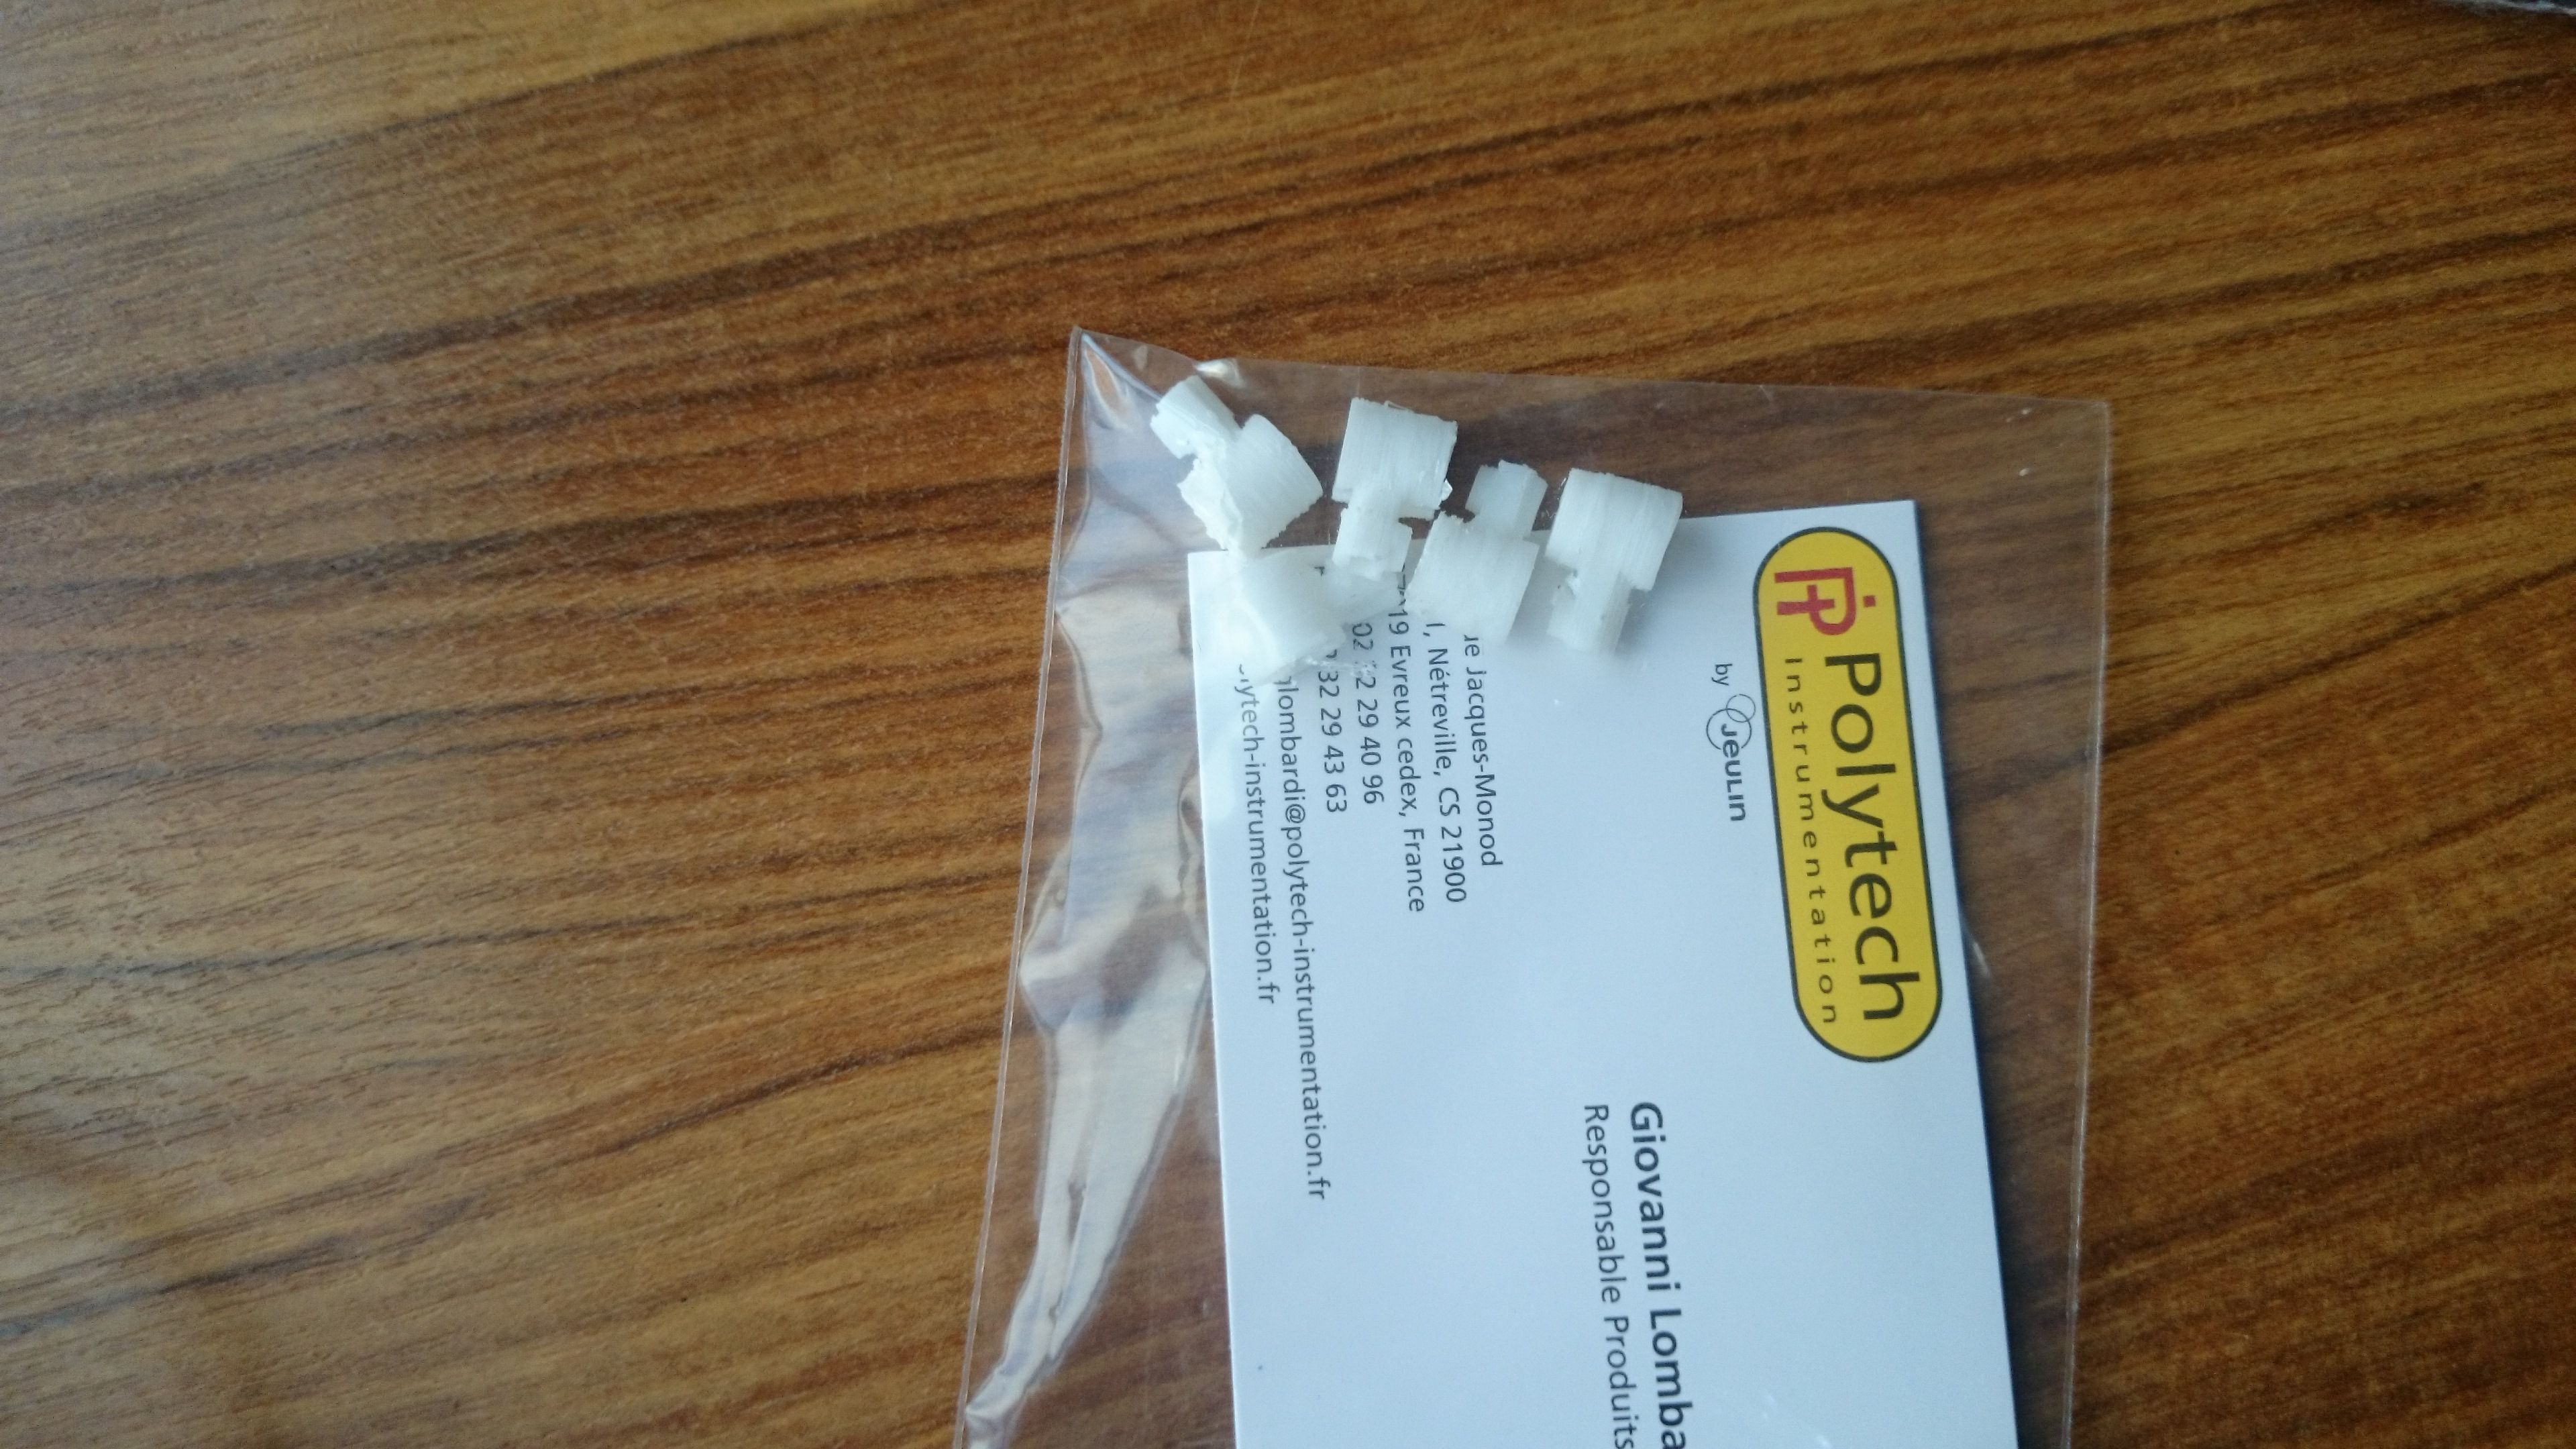
\includegraphics[scale = 0.1]{img/fixations.jpg}
	\caption{Photographie des fixations moteur}
	\label{fixation}
      \end{figure}

      Une fois les fixations moteur en notre possession, il ne nous manquait 
plus que le circuit pour assembler le tout. Pour la production de ce dernier 
nous avons eu l'idée de nous tourner vers l'\textit{ENSEA} qui est une école 
d'ingénieur en électronique proche de la nôtre. Nous leur avons fournit les 
fichiers généré par Fritzing puis ils ont lancé la production. Quelques jours 
plus tard nous avons pu aller récupérer notre circuit. Cependant, il restait 
encore quelques modifications à faire dessus, afin qu'il soit vraiment 
opérationel. En effet, il fallait encore le découper afin d'y créer des embouts 
pour les fixations moteurs. Pour cela nous avons fait appel à une connaissance 
qui dispose des outils nécessaires pour ce genre de situations. Il en a aussi 
profité pour retravailler un peu, à l'aide d'une fraiseuse, les fixations qui 
étaient un peu trop petites. La Figure \ref{circuit} est une photographie de 
notre carte avant et après découpe.

	\begin{figure}[htbp]
	  \begin{subfigure}{.5\textwidth}
	    \centering
	    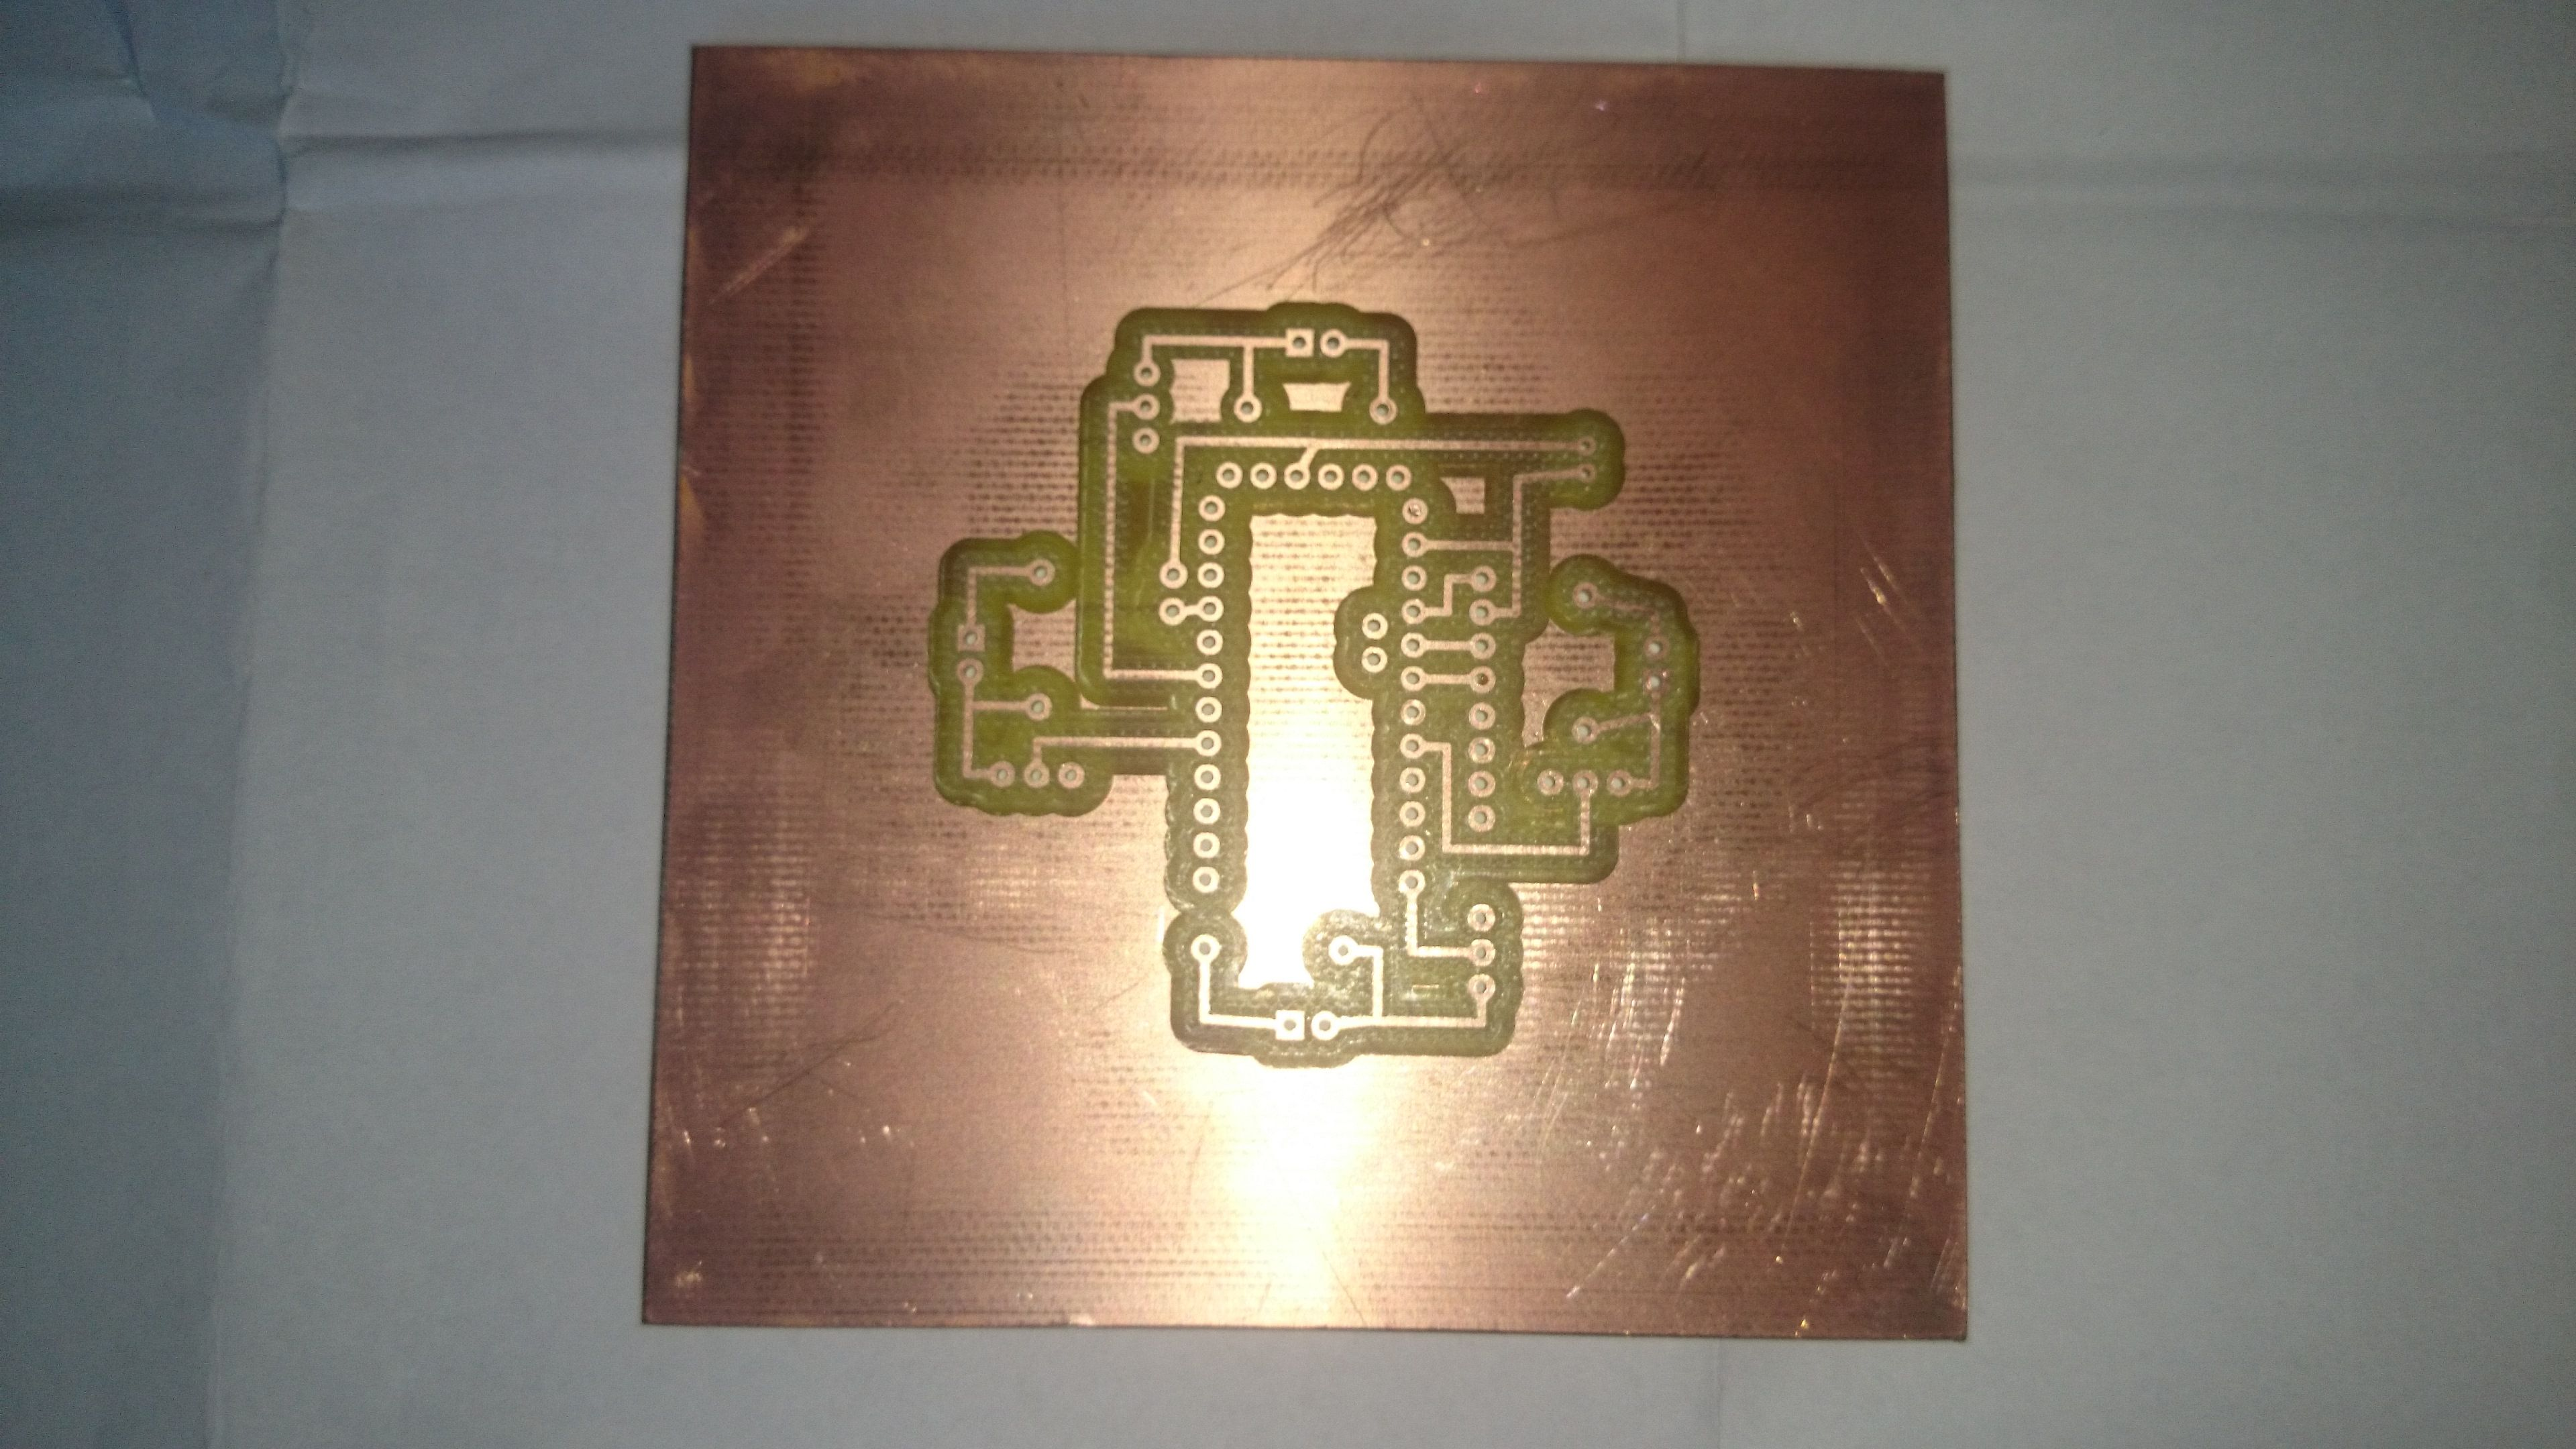
\includegraphics[scale=0.07]{img/carte_avant.jpg}
	    \caption{avant}
	    \label{circuitavant}
	  \end{subfigure}%
	  \begin{subfigure}{.5\textwidth}
	    \centering
	    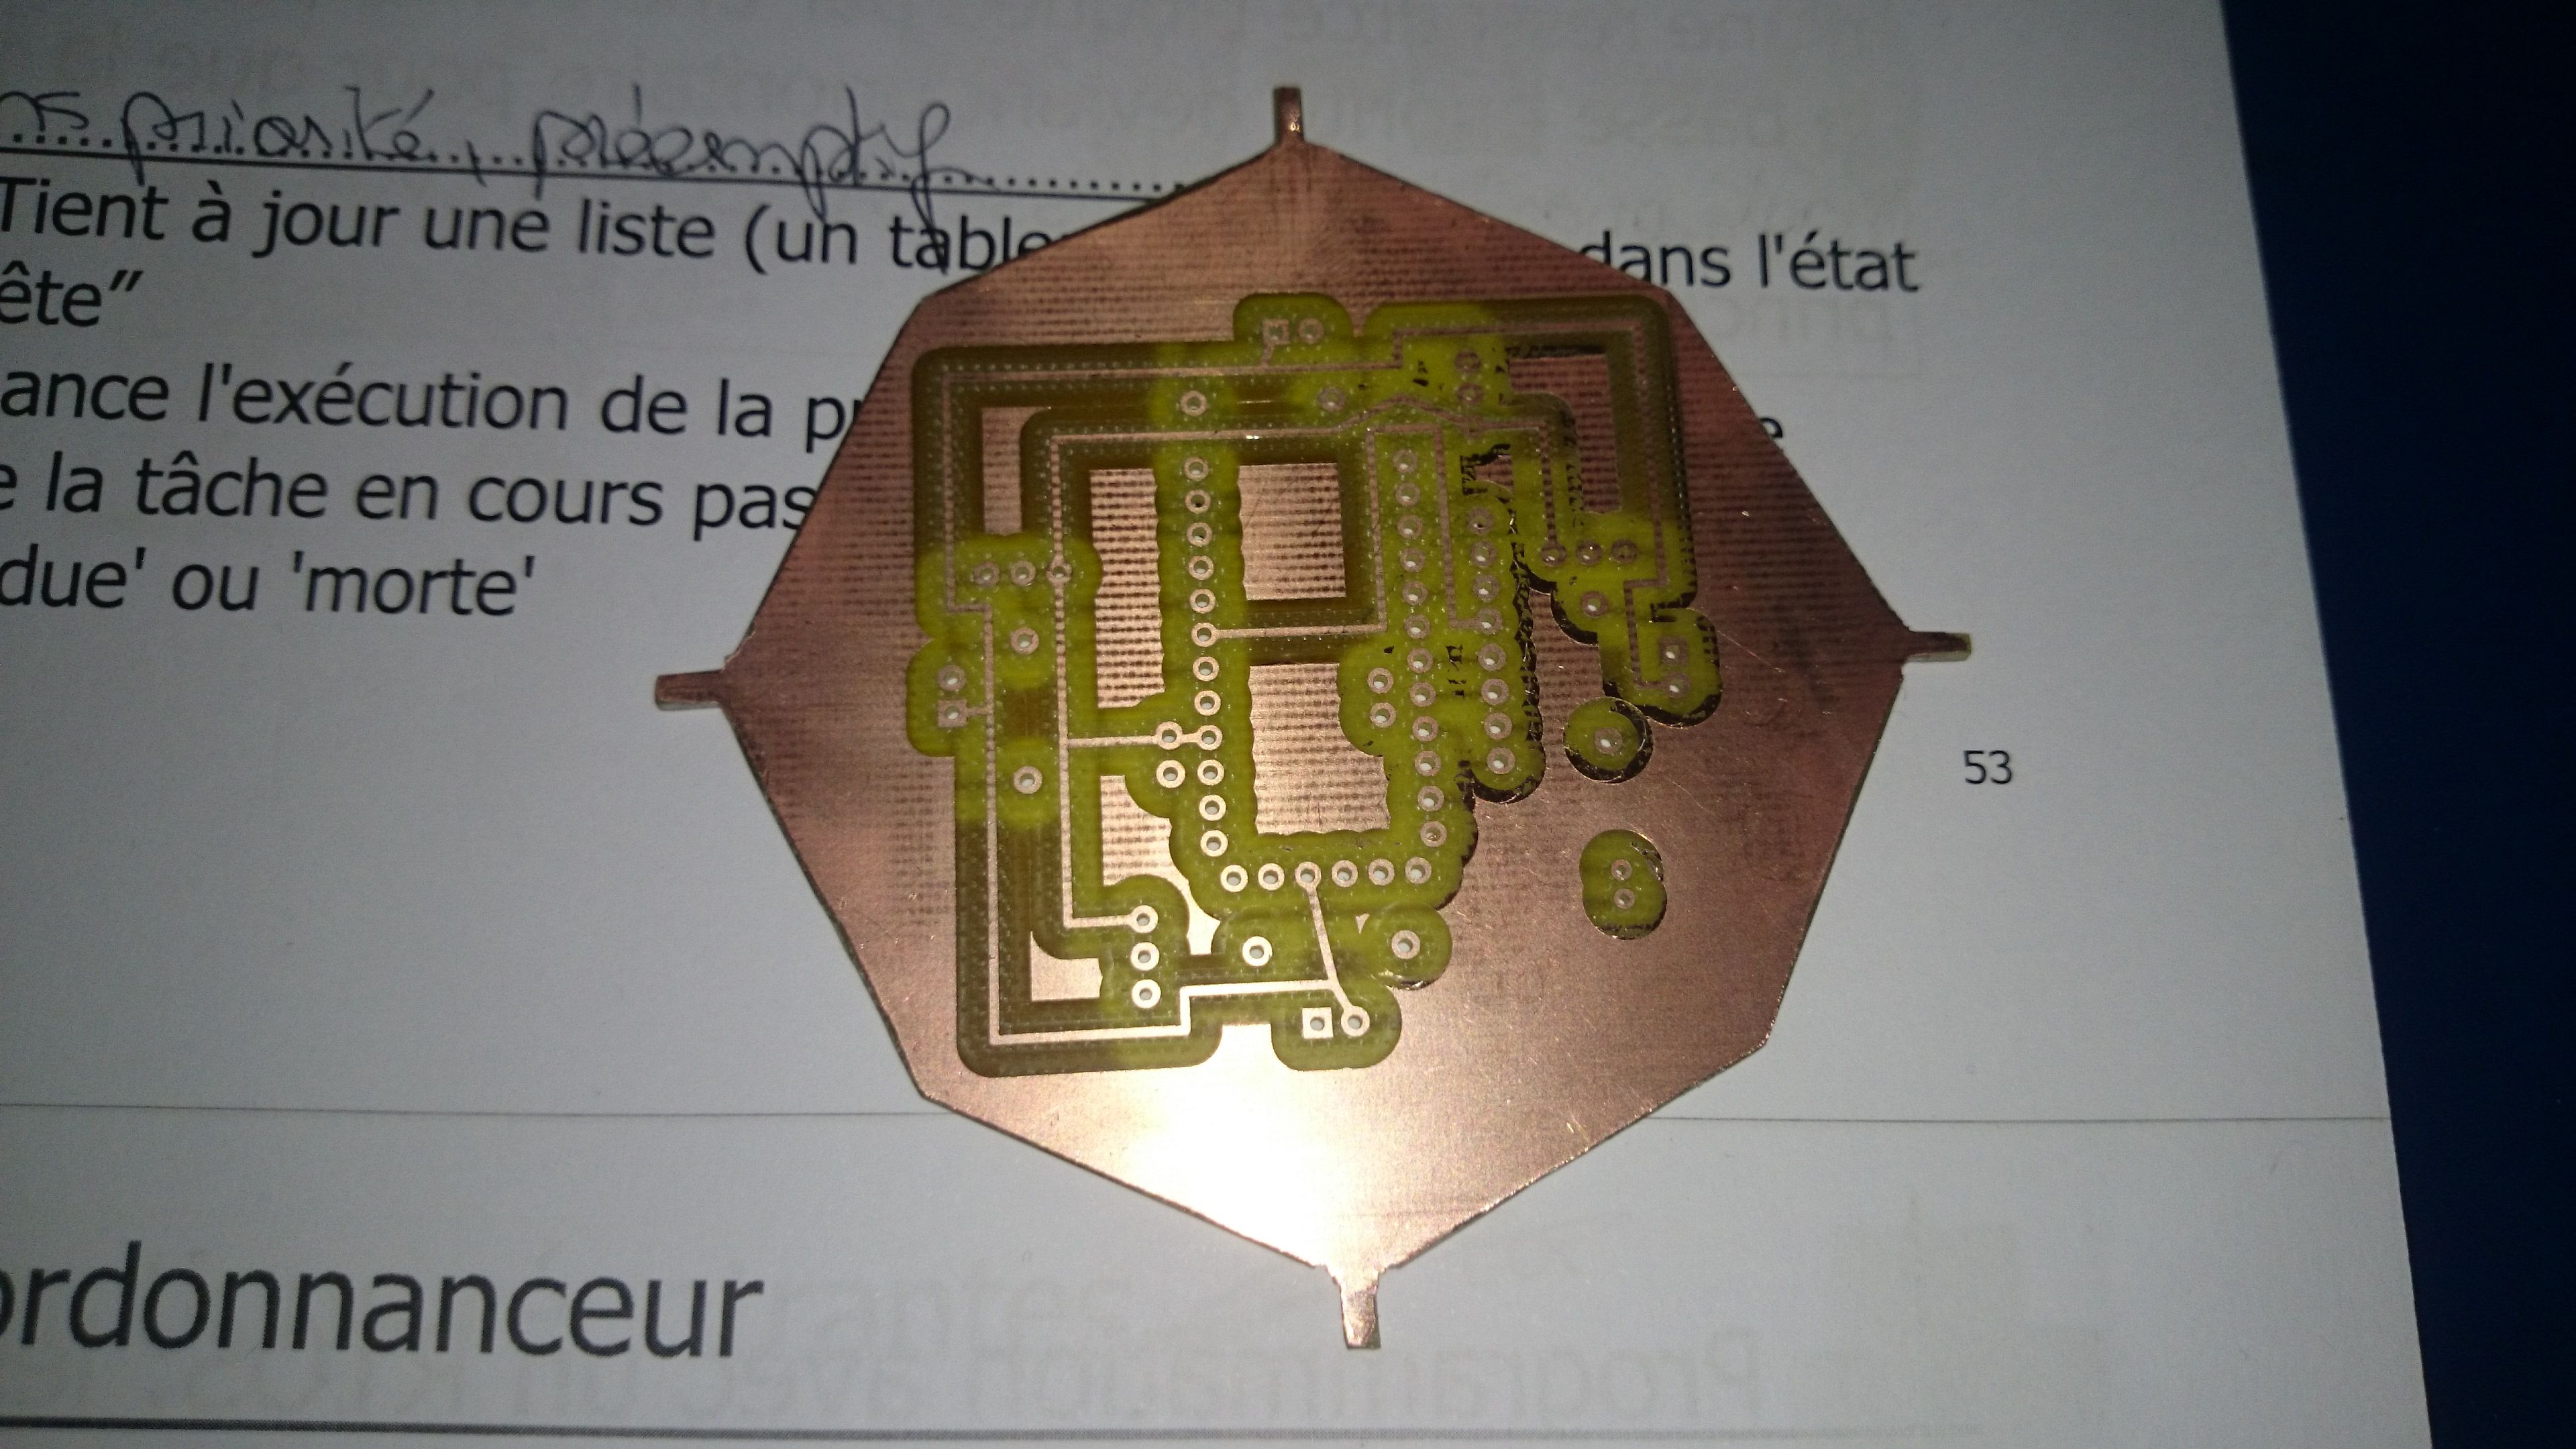
\includegraphics[scale=0.07]{img/carte_apres.jpg}
	    \caption{après}
	    \label{circuitapres}
	  \end{subfigure}
	  \caption{Photographie de notre circuit avant et après découpe}
	  \label{circuit}
	\end{figure}
      
	\subsection{Fabrication et premiers essais}
	  Une fois les deux pièces manquantes rassemblées nous avons pu passer 
à l'assemblage du drone. Nous avons donc soudé les composants sur le circuit et 
collé les fixations. Il est important de noter qu'au moment de l'assemblage 
nous avons constaté que l'Arduino que nous avions achetée n'était pas conforme 
au modèle officiel. En effet, les broches de l'alimentation étaient inversées. 
Par conséquent, notre circuit ne pouvait pas fonctionner. Nous avons dû 
racheter d'urgence une Arduino (cette fois-ci, officielle). Ce problème nous 
aura fait perdre une semaine de travail. La Figure \ref{droneres} est une 
photographie du résultat final.

	  \begin{figure}[htbp]
	    \centering
	    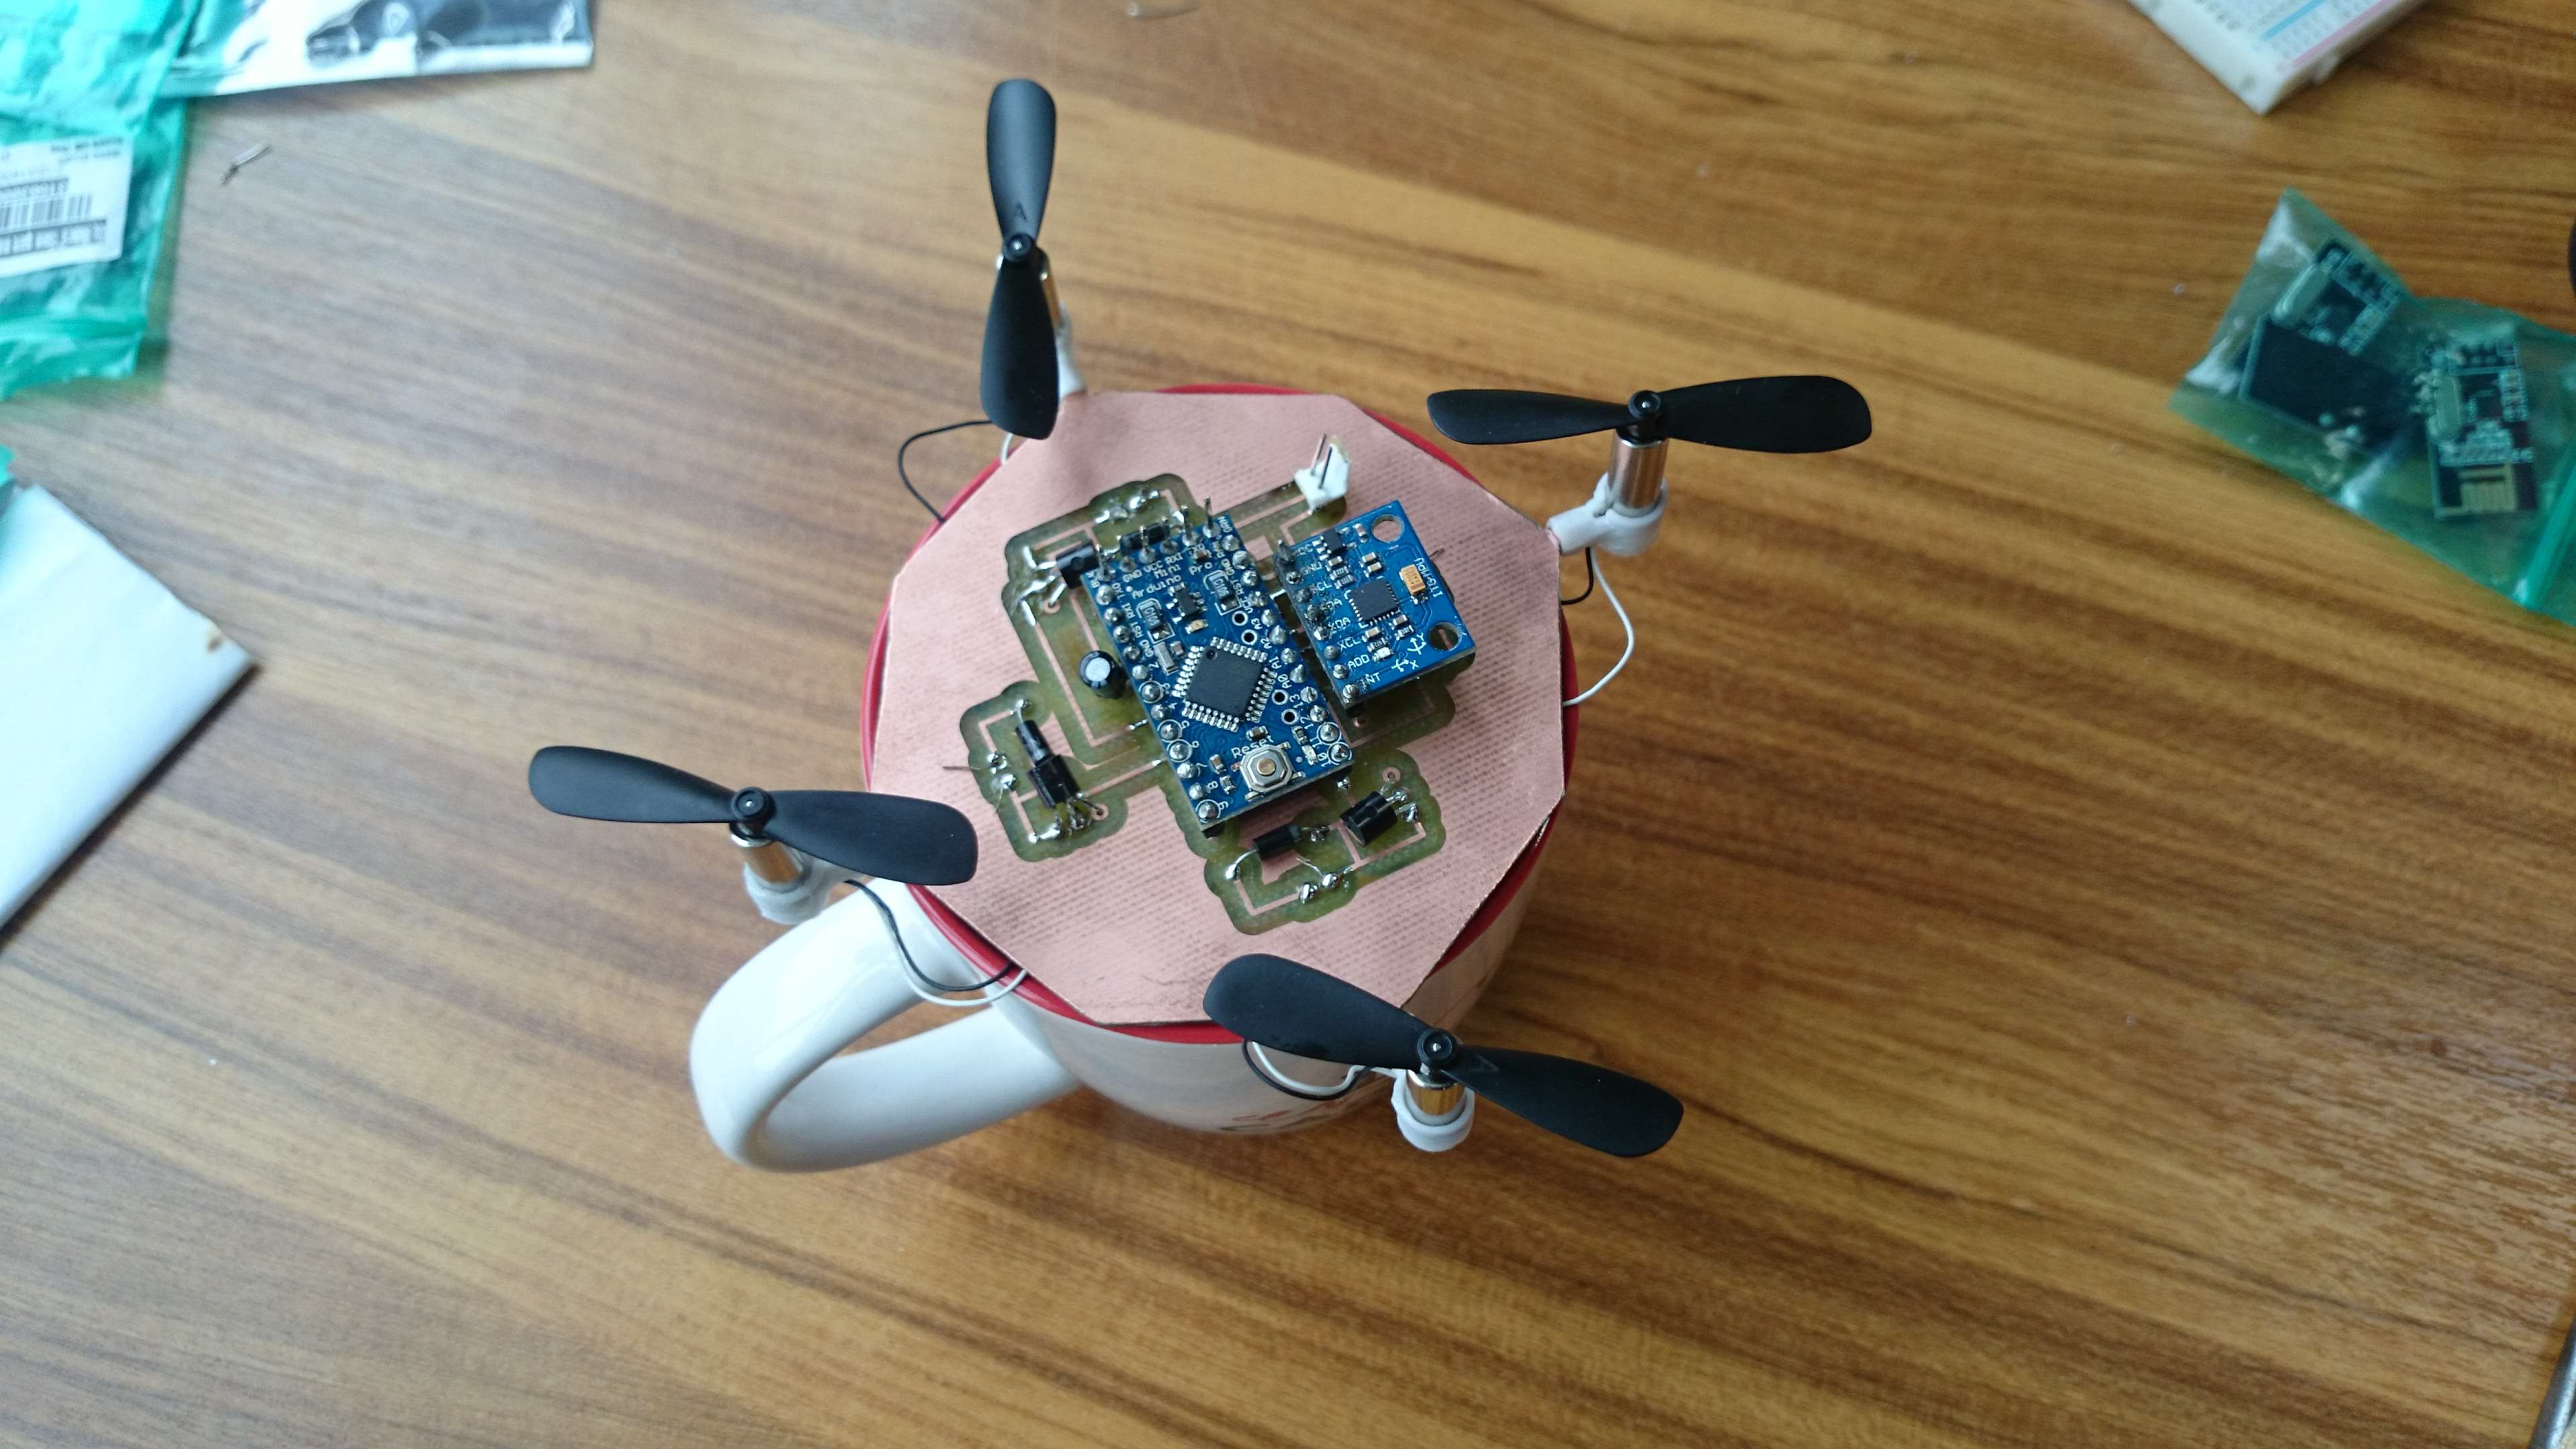
\includegraphics[scale = 0.1]{img/drone_photo.jpg}
	    \caption{Photographie du résultat final}
	    \label{droneres}
	  \end{figure}
	
	  Lorsque nous avons enfin terminé d'assembler le drone notre premier 
réflexe a été de vérifier s'il pouvait décoller. Nous avons alors pour cela 
écrit simple code Arduino qui se contentait de faire tourner les moteurs à 
mi-régime. Sans grande surprise cela ne suffisait pas à le faire décoller. Nous 
avons alors essayé de les faire tourner à plein régime. Et nous avons pu 
constater un problème. Lorsque l'Arduino délivre sa puissance maximum, les 
moteurs ne tournent pas au maximum de leur capacité. En d'autres termes, 
l'Arduino n'est pas capable de délivrer assez de courant pour faire tourner les 
moteurs au maximum de leur capacité. Le drone n'a donc pas décollé.

	  Nous avons eu ensuite une deuxième idée pour tester le décollage. 
Faire un "by-pass" de l'Arduino. C'est à dire brancher les moteurs directement 
sur l'alimentation. En procédant de cette façon les moteurs tournent bien au 
maximum de leur capacité. Mais nous avons constaté un deuxième problème. Un 
moteur est défectueux. Ainsi, lors de notre premier essai sans passer par 
l'Arduino le drone s'est soulevé d'un côté mais le manque de couple produit par 
le moteur défectueux à fait que le drone s'est retourné.

	  Nous pensons donc que si nous possédions quatre moteurs en bon état, 
le drone serait capable de décoller si on les branche directement sur 
l'alimentation. Cependant, ce ne serait pas vraiment intéressant car on ne 
pourrait pas contrôler leur vitesse. Ainsi, le drone ne pourrait que s'élever 
verticalement. Nous ne pourrions pas le faire avancer ou aller sur les côtés. 
De plus on serait dans l'incapacité de le faire s'arrêter.

	  Nous avons alors compris que nous ne pourris pas faire décoller ce 
prototype. De plus, la soutenance approchait à grand pas. Nous n'étions qu'à 
deux semaines de la présentation alors nous n'avions pas le temps de préparer un 
second drone à partir d'autres composants. Nous avons toutefois préparé un code 
pour la présentation, qui servait à montré l'influence du gyroscope sur le 
contrôle des moteurs. Lorsqu'on incline le drone, on peut voir que certains 
moteurs réagissent à cette inclinaison afin d'essayer le stabiliser. Par 
exemple, si on penche le drone vers l'avant, les moteurs avant vont accélérer 
afin d'essayer de replacer le drone parallèlement au sol. De plus on peut 
remarquer que plus l'angle d'inclinaison est important, plus les moteurs 
accélère afin de produire plus de puissance pour essayer de stabiliser 
l'appareil.

  \chapter{Analyse}
  
  
  \chapter{Deuxième drone}
  
  \chapter{Conclusion}
  	   Avec les technologies choisies, nous nous en sortons pour environ 23 
\euro \space de composants pour un drone. Le kit complet du crazyflie coûte à 
peu près 120 \euro. Nous comptions sur le fait que notre drone soit plus lourd 
(environ 35 grammes) que le \textit{Crazyflie} (19 grammes) pour se ramener à 
un vol un peu moins agressif. Aussi la batterie utilisée n'est pas
      intéressante en terme d'autonomie et fournit une tension de 3.3 Volts. 
Cependant les capteurs ultrason que nous comptions utiliser
      fonctionnent en 5 volts. Il nous a donc fallu changer aussi de batterie, 
ce qui nous a obligé à revoir beaucoup de choses. Car le type
      de batterie qu'il nous faut est plus lourd, ce qui implique de changer 
les 
moteurs. Ceci nous entraîne à la création d'un deuxième
      drone.
  
  \appendix
    \chapter{Suivi de projet}
      \section{Gestionnaire de version}
	Pour ce projet nous avons choisi de former un groupe de trois 
personnes. Travailler en équipe a ses avantages, notamment pour le partage de 
tâches. Mais ceci peut entraîner des   problèmes de version entre les travaux de 
chacun. Pour palier ce problème nous avons choisi d'utiliser le gestionnaire 
de version Git. Cet outil est vraiment pratique, puisqu'il permet de travailler 
à distance, de mettre à jour le code de chacun des membres, d'avoir un suivi de 
chaque implémentation, de faire des versions tests (sans toucher à la version 
fonctionnelle) ou encore de revenir à des versions précédentes du projet. Aussi 
cet outil nous permet de donner une visibilité à notre travail. Ainsi, si une 
personne compte faire un projet semblable au nôtre il pourra consulter, 
reprendre, modifier, améliorer... ce que nous avons fait. Notre répertoire Git 
est accéssible depuis cette adresse\cite{njordgit}.
	
      \section{Communication}
	Dès le début du projet nous avons pensé qu'il serait intéressant de 
tenir un blog\cite{njordblog} pour communiquer notre progression. Lorsque l'on 
se lance dans un projet de cette envergure il est toujours utile de trouver 
des ressources sur Internet. Cela peut donner des idées et résoudre des 
problématiques que l'on rencontre. Afin de pouvoir communiquer avec le plus de 
monde possible, il est rédigé dans trois langues : anglais, français et 
japonais. Il présente l'avancée du projet, nos choix de développement, quelques 
notions de physique et les résultats de nos essais afin de guider les lecteur 
qui veulent créer une application similaire. Nous avons souhaité présenter le 
processus de construction d'un drone, sous une forme simple, en expliquant 
comment les choses fonctionnent.
	
    \chapter{Fonctionnement d'un gyroscope}

  \listoffigures
  
  \raggedright
  \bibliographystyle{unsrt}
  \bibliography{biblio}
\end{document}          
